%% bare_conf_compsoc.tex
%% V1.4b
%% 2015/08/26
%% by Michael Shell
%% See:
%% http://www.michaelshell.org/
%% for current contact information.
%%
%% This is a skeleton file demonstrating the use of IEEEtran.cls
%% (requires IEEEtran.cls version 1.8b or later) with an IEEE Computer
%% Society conference paper.
%%
%% Support sites:
%% http://www.michaelshell.org/tex/ieeetran/
%% http://www.ctan.org/pkg/ieeetran
%% and
%% http://www.ieee.org/

\documentclass[conference,compsoc]{IEEEtran}
% Some/most Computer Society conferences require the compsoc mode option,
% but others may want the standard conference format.
%
% If IEEEtran.cls has not been installed into the LaTeX system files,
% manually specify the path to it like:
% \documentclass[conference,compsoc]{../sty/IEEEtran}

% *** MISC UTILITY PACKAGES ***
%
\usepackage{ifpdf}
\usepackage{framed}
% Heiko Oberdiek's ifpdf.sty is very useful if you need conditional
% compilation based on whether the output is pdf or dvi.
% usage:
% \ifpdf
%   % pdf code
% \else
%   % dvi code
% \fi
% The latest version of ifpdf.sty can be obtained from:
% http://www.ctan.org/pkg/ifpdf
% Also, note that IEEEtran.cls V1.7 and later provides a builtin
% \ifCLASSINFOpdf conditional that works the same way.
% When switching from latex to pdflatex and vice-versa, the compiler may
% have to be run twice to clear warning/error messages.



% *** CITATION PACKAGES ***
%
\ifCLASSOPTIONcompsoc
  % IEEE Computer Society needs nocompress option
  % requires cite.sty v4.0 or later (November 2003)
  \usepackage[nocompress]{cite}
\else
  % normal IEEE
  \usepackage{cite}
\fi



% *** GRAPHICS RELATED PACKAGES ***
%
\ifCLASSINFOpdf
  % \usepackage[pdftex]{graphicx}
  % declare the path(s) where your graphic files are
  % \graphicspath{{../pdf/}{../jpeg/}}
  % and their extensions so you won't have to specify these with
  % every instance of \includegraphics
  % \DeclareGraphicsExtensions{.pdf,.jpeg,.png}
\else
  % or other class option (dvipsone, dvipdf, if not using dvips). graphicx
  % will default to the driver specified in the system graphics.cfg if no
  % driver is specified.
  % \usepackage[dvips]{graphicx}
  % declare the path(s) where your graphic files are
  % \graphicspath{{../eps/}}
  % and their extensions so you won't have to specify these with
  % every instance of \includegraphics
  % \DeclareGraphicsExtensions{.eps}
\fi
% graphicx was written by David Carlisle and Sebastian Rahtz. It is
% required if you want graphics, photos, etc. graphicx.sty is already
% installed on most LaTeX systems. The latest version and documentation
% can be obtained at: 
% http://www.ctan.org/pkg/graphicx
% Another good source of documentation is "Using Imported Graphics in
% LaTeX2e" by Keith Reckdahl which can be found at:
% http://www.ctan.org/pkg/epslatex
%
% latex, and pdflatex in dvi mode, support graphics in encapsulated
% postscript (.eps) format. pdflatex in pdf mode supports graphics
% in .pdf, .jpeg, .png and .mps (metapost) formats. Users should ensure
% that all non-photo figures use a vector format (.eps, .pdf, .mps) and
% not a bitmapped formats (.jpeg, .png). The IEEE frowns on bitmapped formats
% which can result in "jaggedy"/blurry rendering of lines and letters as
% well as large increases in file sizes.
%
% You can find documentation about the pdfTeX application at:
% http://www.tug.org/applications/pdftex





% *** MATH PACKAGES ***
%
\usepackage{amsmath}
\usepackage{cuted}
% A popular package from the American Mathematical Society that provides
% many useful and powerful commands for dealing with mathematics.
%
% Note that the amsmath package sets \interdisplaylinepenalty to 10000
% thus preventing page breaks from occurring within multiline equations. Use:
%\interdisplaylinepenalty=2500
% after loading amsmath to restore such page breaks as IEEEtran.cls normally
% does. amsmath.sty is already installed on most LaTeX systems. The latest
% version and documentation can be obtained at:
% http://www.ctan.org/pkg/amsmath
\newcommand\numberthis{\addtocounter{equation}{1}\tag{\theequation}}




% *** SPECIALIZED LIST PACKAGES ***
%
\usepackage{algorithmic}
% algorithmic.sty was written by Peter Williams and Rogerio Brito.
% This package provides an algorithmic environment fo describing algorithms.
% You can use the algorithmic environment in-text or within a figure
% environment to provide for a floating algorithm. Do NOT use the algorithm
% floating environment provided by algorithm.sty (by the same authors) or
% algorithm2e.sty (by Christophe Fiorio) as the IEEE does not use dedicated
% algorithm float types and packages that provide these will not provide
% correct IEEE style captions. The latest version and documentation of
% algorithmic.sty can be obtained at:
% http://www.ctan.org/pkg/algorithms
% Also of interest may be the (relatively newer and more customizable)
% algorithmicx.sty package by Szasz Janos:
% http://www.ctan.org/pkg/algorithmicx




% *** ALIGNMENT PACKAGES ***
%
\usepackage{array}
% Frank Mittelbach's and David Carlisle's array.sty patches and improves
% the standard LaTeX2e array and tabular environments to provide better
% appearance and additional user controls. As the default LaTeX2e table
% generation code is lacking to the point of almost being broken with
% respect to the quality of the end results, all users are strongly
% advised to use an enhanced (at the very least that provided by array.sty)
% set of table tools. array.sty is already installed on most systems. The
% latest version and documentation can be obtained at:
% http://www.ctan.org/pkg/array


% IEEEtran contains the IEEEeqnarray family of commands that can be used to
% generate multiline equations as well as matrices, tables, etc., of high
% quality.




% *** SUBFIGURE PACKAGES ***
%\ifCLASSOPTIONcompsoc
%  \usepackage[caption=false,font=footnotesize,labelfont=sf,textfont=sf]{subfig}
%\else
%  \usepackage[caption=false,font=footnotesize]{subfig}
%\fi
% subfig.sty, written by Steven Douglas Cochran, is the modern replacement
% for subfigure.sty, the latter of which is no longer maintained and is
% incompatible with some LaTeX packages including fixltx2e. However,
% subfig.sty requires and automatically loads Axel Sommerfeldt's caption.sty
% which will override IEEEtran.cls' handling of captions and this will result
% in non-IEEE style figure/table captions. To prevent this problem, be sure
% and invoke subfig.sty's "caption=false" package option (available since
% subfig.sty version 1.3, 2005/06/28) as this is will preserve IEEEtran.cls
% handling of captions.
% Note that the Computer Society format requires a sans serif font rather
% than the serif font used in traditional IEEE formatting and thus the need
% to invoke different subfig.sty package options depending on whether
% compsoc mode has been enabled.
%
% The latest version and documentation of subfig.sty can be obtained at:
% http://www.ctan.org/pkg/subfig
\usepackage{verbatim}
\usepackage{soul}
\usepackage{xcolor}
\newcommand{\TODO}[1]{\hl{TODO: #1}}
\newcommand{\NOTE}[1]{\hl {NOTE: #1}}
\newcommand{\changed}[1]{\textcolor{red}{#1}}


% *** FLOAT PACKAGES ***
%
%\usepackage{fixltx2e}
% fixltx2e, the successor to the earlier fix2col.sty, was written by
% Frank Mittelbach and David Carlisle. This package corrects a few problems
% in the LaTeX2e kernel, the most notable of which is that in current
% LaTeX2e releases, the ordering of single and double column floats is not
% guaranteed to be preserved. Thus, an unpatched LaTeX2e can allow a
% single column figure to be placed prior to an earlier double column
% figure.
% Be aware that LaTeX2e kernels dated 2015 and later have fixltx2e.sty's
% corrections already built into the system in which case a warning will
% be issued if an attempt is made to load fixltx2e.sty as it is no longer
% needed.
% The latest version and documentation can be found at:
% http://www.ctan.org/pkg/fixltx2e


%\usepackage{stfloats}
% stfloats.sty was written by Sigitas Tolusis. This package gives LaTeX2e
% the ability to do double column floats at the bottom of the page as well
% as the top. (e.g., "\begin{figure*}[!b]" is not normally possible in
% LaTeX2e). It also provides a command:
%\fnbelowfloat
% to enable the placement of footnotes below bottom floats (the standard
% LaTeX2e kernel puts them above bottom floats). This is an invasive package
% which rewrites many portions of the LaTeX2e float routines. It may not work
% with other packages that modify the LaTeX2e float routines. The latest
% version and documentation can be obtained at:
% http://www.ctan.org/pkg/stfloats
% Do not use the stfloats baselinefloat ability as the IEEE does not allow
% \baselineskip to stretch. Authors submitting work to the IEEE should note
% that the IEEE rarely uses double column equations and that authors should try
% to avoid such use. Do not be tempted to use the cuted.sty or midfloat.sty
% packages (also by Sigitas Tolusis) as the IEEE does not format its papers in
% such ways.
% Do not attempt to use stfloats with fixltx2e as they are incompatible.
% Instead, use Morten Hogholm'a dblfloatfix which combines the features
% of both fixltx2e and stfloats:
%
% \usepackage{dblfloatfix}
% The latest version can be found at:
% http://www.ctan.org/pkg/dblfloatfix




% *** PDF, URL AND HYPERLINK PACKAGES ***
%
\usepackage{url}
% url.sty was written by Donald Arseneau. It provides better support for
% handling and breaking URLs. url.sty is already installed on most LaTeX
% systems. The latest version and documentation can be obtained at:
% http://www.ctan.org/pkg/url
% Basically, \url{my_url_here}.

\usepackage{graphicx} % Required for including pictures
\graphicspath{{pics/}} % Specifies the directory where pictures are stored
\usepackage{caption}
\usepackage{subcaption}
\usepackage{booktabs}
\usepackage{multirow} % make table

\makeatletter % Put Roman Number in Text
\newcommand{\rmnum}[1]{\romannumeral #1}
\newcommand{\Rmnum}[1]{\expandafter\@slowromancap\romannumeral #1@}
\makeatother



% *** Do not adjust lengths that control margins, column widths, etc. ***
% *** Do not use packages that alter fonts (such as pslatex).         ***
% There should be no need to do such things with IEEEtran.cls V1.6 and later.
% (Unless specifically asked to do so by the journal or conference you plan
% to submit to, of course. )


% correct bad hyphenation here
\hyphenation{op-tical net-works semi-conduc-tor}


\begin{document}
%
% paper title
% Titles are generally capitalized except for words such as a, an, and, as,
% at, but, by, for, in, nor, of, on, or, the, to and up, which are usually
% not capitalized unless they are the first or last word of the title.
% Linebreaks \\ can be used within to get better formatting as desired.
% Do not put math or special symbols in the title.
\title{Watch Out for the Bully! Study of Interference Between Jobs Running Concurrently on Dragonfly Network}


% author names and affiliations
% use a multiple column layout for up to three different
% affiliations
% \author{\IEEEauthorblockN{Michael Shell}
% \IEEEauthorblockA{School of Electrical and\\Computer Engineering\\
% Georgia Institute of Technology\\
% Atlanta, Georgia 30332--0250\\
% Email: http://www.michaelshell.org/contact.html}
% \and
% \IEEEauthorblockN{Homer Simpson}
% \IEEEauthorblockA{Twentieth Century Fox\\
% Springfield, USA\\
% Email: homer@thesimpsons.com}
% \and
% \IEEEauthorblockN{James Kirk\\ and Montgomery Scott}
% \IEEEauthorblockA{Starfleet Academy\\
% San Francisco, California 96678-2391\\
% Telephone: (800) 555--1212\\
% Fax: (888) 555--1212}}


\author{

\IEEEauthorblockN{Xu Yang\IEEEauthorrefmark{1}, John Jenkins\IEEEauthorrefmark{2}, Misbah Mubarak\IEEEauthorrefmark{2}, Robert B. Ross\IEEEauthorrefmark{2}, Zhiling Lan\IEEEauthorrefmark{1}}

\IEEEauthorblockA{\IEEEauthorrefmark{1}Department of Computer Science,
Illinois Institute of Technology,
Chicago, Illinois, USA 60616\\
\{xyang56\}@hawk.iit.edu, lan@iit.edu}

\IEEEauthorblockA{\IEEEauthorrefmark{2}Mathematics and Computer Science Division, Argonne National Laboratory,
Argonne, IL, USA 60439\\
\{jenkins,rross\}@mcs.anl.gov, mmubarak@anl.gov}
}


% conference papers do not typically use \thanks and this command
% is locked out in conference mode. If really needed, such as for
% the acknowledgment of grants, issue a \IEEEoverridecommandlockouts
% after \documentclass

% for over three affiliations, or if they all won't fit within the width
% of the page (and note that there is less available width in this regard for
% compsoc conferences compared to traditional conferences), use this
% alternative format:
% 
%\author{\IEEEauthorblockN{Michael Shell\IEEEauthorrefmark{1},
%Homer Simpson\IEEEauthorrefmark{2},
%James Kirk\IEEEauthorrefmark{3}, 
%Montgomery Scott\IEEEauthorrefmark{3} and
%Eldon Tyrell\IEEEauthorrefmark{4}}
%\IEEEauthorblockA{\IEEEauthorrefmark{1}School of Electrical and Computer Engineering\\
%Georgia Institute of Technology,
%Atlanta, Georgia 30332--0250\\ Email: see http://www.michaelshell.org/contact.html}
%\IEEEauthorblockA{\IEEEauthorrefmark{2}Twentieth Century Fox, Springfield, USA\\
%Email: homer@thesimpsons.com}
%\IEEEauthorblockA{\IEEEauthorrefmark{3}Starfleet Academy, San Francisco, California 96678-2391\\
%Telephone: (800) 555--1212, Fax: (888) 555--1212}
%\IEEEauthorblockA{\IEEEauthorrefmark{4}Tyrell Inc., 123 Replicant Street, Los Angeles, California 90210--4321}}




% use for special paper notices
%\IEEEspecialpapernotice{(Invited Paper)}




% make the title area
\maketitle

% As a general rule, do not put math, special symbols or citations
% in the abstract
\begin{abstract}

The high-radix, low-diameter dragonfly topology network will be the choice of many computing facilities for building their next generation supercomputers. Preliminary study shows that random placement with adaptive routing should be the rule of thumb to utilize such powerful network, since random placement can uniformly distribut traffic over the network, and adaptive routing can alleviate congestion. However, in this paper, we made the observation that although random placement coupled with adaptive routing can reach load-balanced over the network when multiple jobs running concurrently, it can not guarantee the best performance for each single job. The performance improvement of communication intensive jobs comes with sacrifice of those less intensive jobs. We refer this phenomenon as ``bully" between concurrently running jobs. We analyze the detailed reason behind this ``bully" behavior between jobs from the underneath network level. Our study is based on a sophisticated, high-fidelity discrete even-driven simulation tool. We believe the observations and analysis in this work will make the chosen of job placement and routing strategies on dragonfly network more cautiously in future.


\end{abstract}

% no keywords

% \keywords{Dragonfly, Job placement, Routing, Interference}



% For peer review papers, you can put extra information on the cover
% page as needed:
% \ifCLASSOPTIONpeerreview
% \begin{center} \bfseries EDICS Category: 3-BBND \end{center}
% \fi
%
% For peerreview papers, this IEEEtran command inserts a page break and
% creates the second title. It will be ignored for other modes.
\IEEEpeerreviewmaketitle



\section{Introduction}
\label{sec:intro}

The low latency and high bandwidth interconnect network plays a critical role in improving HPC system performance. As the computing ability continue to grow due to many-core nodes with accelerators, the network is now becoming a scare resources. HPC community start to explore the new network topology to replace the commonly used torus-connected network. The high-radix, low-diameter dragonfly topology can lower the cost of interconnect network, improve network bandwidth, reduce the packets traverse latency \cite{dally-dragonfly}. This make the dragonfly network an very promising choice for building Petaflop and beyond supercomputers. 
%The procurement results from Trinity and CORAL project shows the great performance improvement can be got from using dragonfly network. 


While dragonfly topology provides low-latency and high-bandwidth interconnected network, how to efficiently utilize it is greatly relying on the upper level system software. In particular, intelligent job placement to avoid interference is of paramount importance for guarantee the performance of concurrently running jobs that sharing network resources \cite{bhatele2015, dskinner}. Some research work suggest that random job placement coupled with adaptive routing can alleviate local congestion, eliminate hot-spots and reach load-balance for dragonfly networks \cite{jain-sc14, bhatele-sc11, brandt2014}. 


In this work, we study the interference between concurrently running jobs on dragonfly network with different job placement and routing schemes. We use CODES, a HPC network simulation toolkit with high fidelity, excellent scalability for packet level simulation \cite{codes}. And being unorthodox to most existing work that use synthetic workload, we use traces of three representative applications from DOE Design Forward Project \cite{designforwardwebpage}. The advantage of using real application traces is quite obvious, these traces can capture application's communication behavior in detail that usually omitted in synthetic workload for the purpose of simplicity. Applications usually are distinctive from each other in terms of data transfer amount, communication pattern, operation dependency etc. which are impossible to reproduce in synthetic workload.

We conduct extensive experiments with three applications running on dragonfly network with two job placement schemes and three routing schemes. We analyze the applications' performance in terms of communication time when they running with different placement\& routing configuration. Our evaluation is based on more than 1000 runs of simulation. Through extensive simulation with application traces, we make several interesting observations. 


%We made observation from our extensive study that, when dragonfly network is configured with random placement and adaptive routing scheme in order to reach hot-spots free and load balance, the performance of particular job(s) in the workload would suffer degradation. The communication intensive jobs in the workload can benefit from random placement and adaptive routing, with great performance improvement. Unfortunately, those less intensive jobs are the sacrifices for this improvement, their performance will be greatly reduced. We identify this phenomenon as ``bully" between concurrently running jobs.

\begin{itemize}
   
    \item Random placement coupled with adaptive routing can not guarantee the performance of every job in the workload. The hot-spots free and load-balanced network status reached by using random placement with adaptive routing come with the cost of less communication-intensive jobs performance degradation. 

    \item We identify the ``bully" behavior happening between concurrently running jobs on dragonfly network when random placement \& adaptive routing in use. Random placement \& adaptive routing redirect the traffic of communication intensive jobs to the routers through which less intensive jobs' traffic used to go, embezzle the network resource such as local and global channel bandwidth, slow down the communication of those less intensive jobs.

    
    \item We found that contiguous placement \& minimal routing can guarantee the consistent performance of each job running on dragonfly network, while may result in local network congestion and unbalanced network utilization. Contiguous placement \& minimal routing are preferred by less communication-intensive jobs, since it will prevent them from being ``bullied" by other communication-intensive jobs.
    
         
\end{itemize}

These observations also reconfirm that interference between concurrently running jobs would make the performance of some jobs very unpredictable. The detailed analysis about the traffic and congestion in network level unveil the undercurrent beneath that interference. 

To the best of our knowledge, using parallel application traces from production systems for the study of job interference on dragonfly network has not been reported so far. We believe the observations and analysis presented in this paper are valuable to a number of communities including HPC computing facility, system software development, and system administration. The computing facility should choose the configuration for dragonfly network implementation with consideration about resource sharing between concurrently running jobs. The workload manager would come up with better scheduling algorithm for jobs with distinctive communication behavior. And the system administration would be more efficient with the knowledge about jobs running status under different placement and routing configuration.

The rest of this paper is organized as follows. Section \ref{sec:background} describes the dragonfly network and the placement \& routing schemes. Section \ref{sec: methodology} talks about the use of CODES as research vehicle and three representative applications from DOE Design Forward Project. Section \ref{sec:workload-1} presents the analysis of three applications running on dragonfly network with different placement \& routing configuration. Section \ref{sec:workload-2} validates the observations we get in section \ref{sec:workload-1}. Section \ref{sec:related work} discusses related work. Finally, the conclusion is presented in Section \ref{sec:conclusion}.

\section{Background}
\label{sec:background}

In this section, we talk about the Dragonfly topology and one of its implementation. We also present the placement and routing schemes  used on dragonfly network.

\subsection{Dragonfly Network}
\label{sec:network}
The dragonfly is a two-level hierarchical topology. It consists of several groups connected by All-to-All links. In each group, there could be ``a" number of routers connected via All-to-All local channels. For each router, there could be ``p" number of compute nodes attached to it via terminal links. The router has ``h" number of global channels that used as intergroup connections through which the router connected to other routers in different groups. Thus, the radix of each router is $k = a+h+p-1$. The implementation of such dragonfly network could be different between different computing facilities. The choosing of proper $a$, $h$, $p$ could be involving many factors, such as system scale, building cost and workload requirements. 

For the purpose of loading balance, it is recommended that the proper dragonfly configuration should be like $a=2p=2h$\cite{kim-micro}. Under this configuration, the total number of groups ``g" in the dragonfly network would be $g = a*h+1 $, the total number of compute nodes ``N" in the network would be $N = p*a*g $. Figure \ref{fig:dragonfly-overview} illustrated an implementation of dragonfly network follows such configuration. There are 6 routers in each group, each router has 3 compute nodes attached to it. This dragonfly implementation consists of 19 groups and 342 nodes in total.

\begin{figure}[h!] 
  \centering
  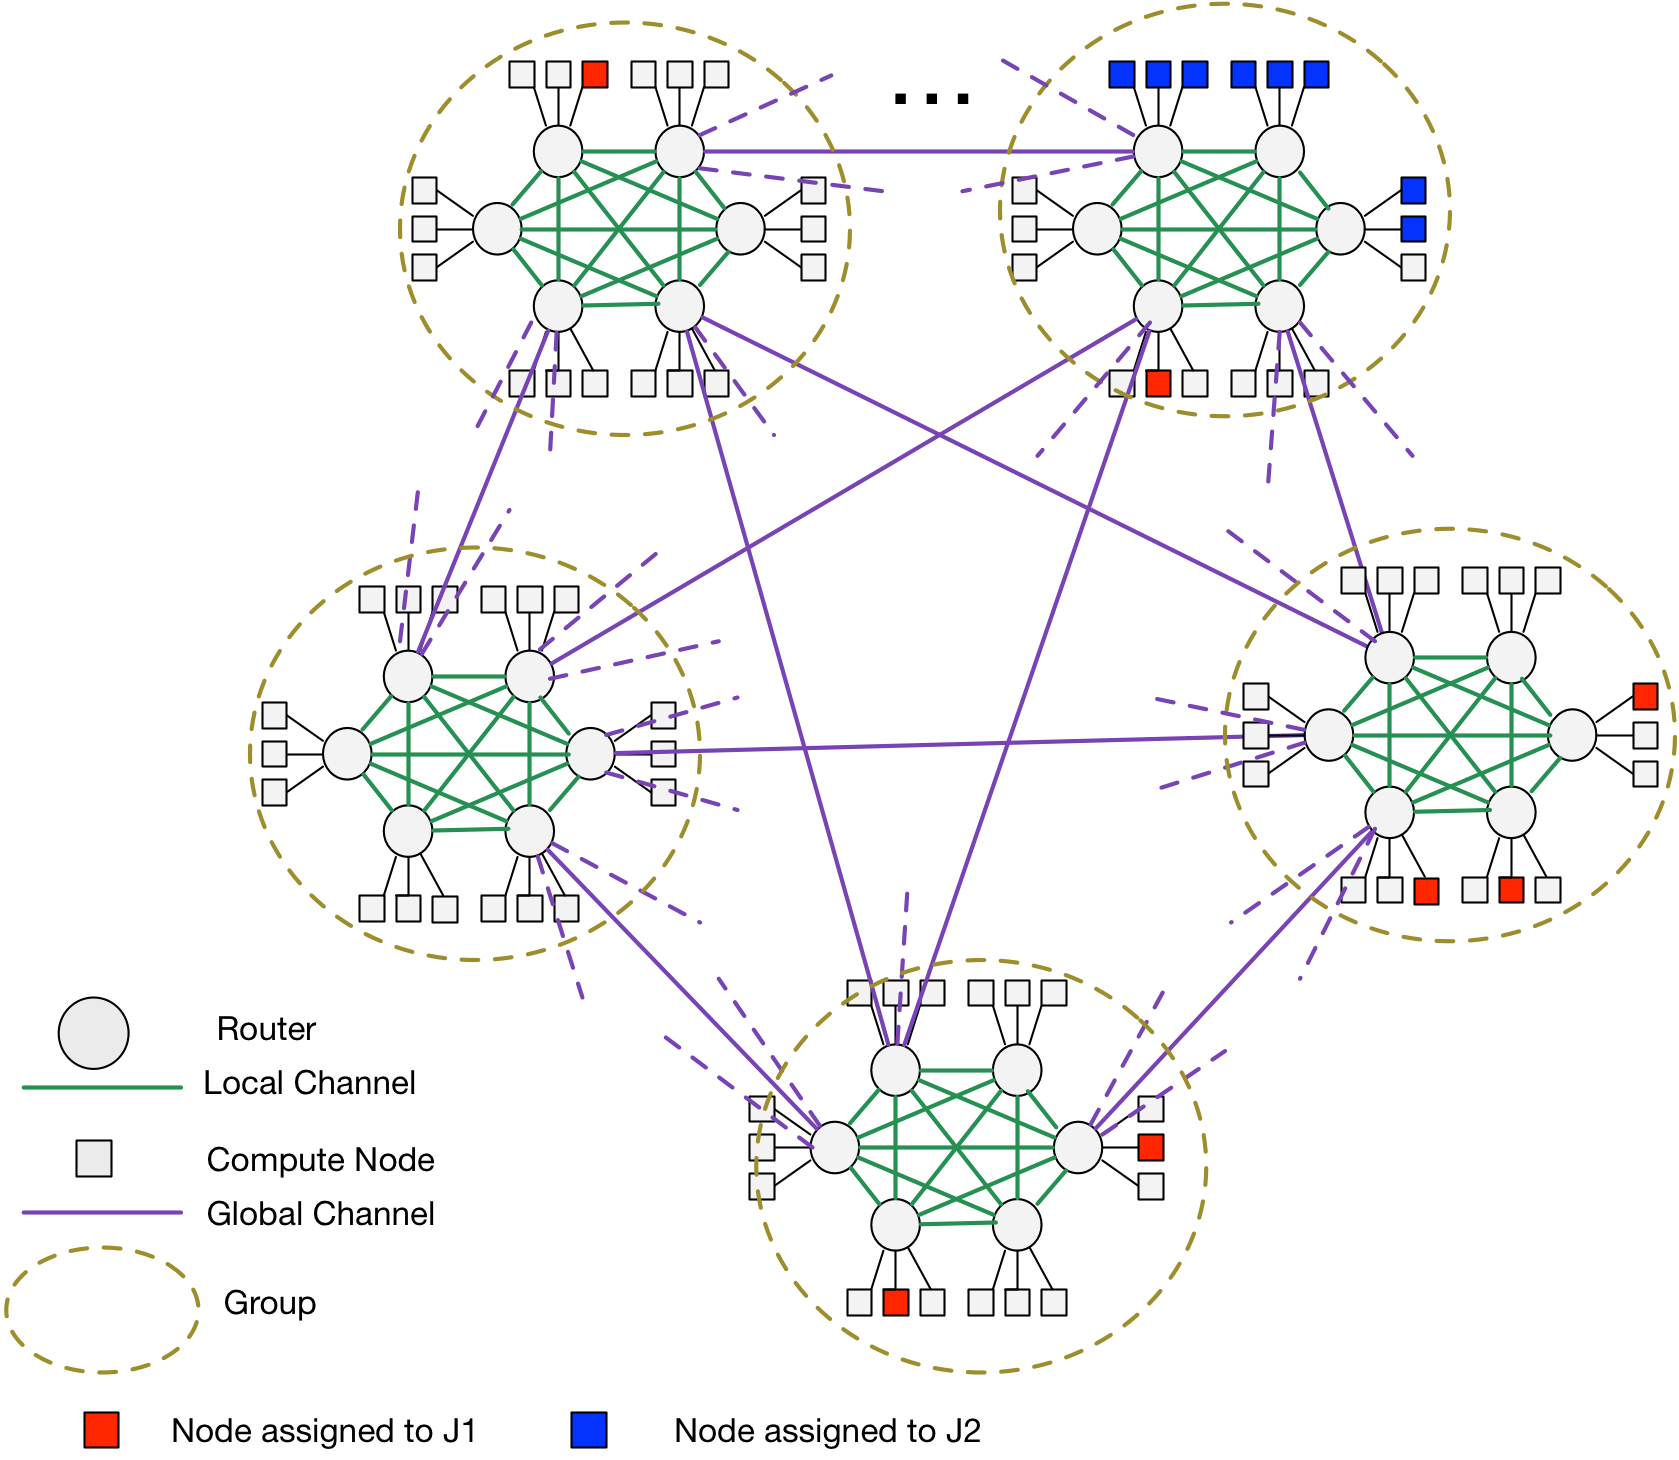
\includegraphics[width=0.48\textwidth]{dragonfly-overview}
  \caption{Dragonfly Network Overview. Illustration of part of dragonfly network. There are 19 groups, 6 routers in each group, 3 compute nodes connected to each router, 342 nodes in total. Job\_1 requires for 6 nodes, get the allocation by Random placement. Job\_2 requires for 8 nodes, get the allocation by Contiguous placement. }
  \label{fig:dragonfly-overview}
\end{figure}


\subsection{Job Placement on Dragonfly}
\label{sec:placement-schemes}

For a parallel application requiring multiple compute nodes, job placement refers to the process of assigning the tasks of the application onto the system by a system software such as batch scheduler \cite{xu-cluster14}. In this work, we study two well cited placement policies for dragonfly systems: 

%Job placement refers to the scheme used by batch scheduler to allocate the required number of nodes by each job for execution. As studied by several researchers, the job placement could be an important factor that impact application performance \cite{hoefler-hpdc14} \cite{bhatele-sc11} \cite{jain-sc14}. In this work, we study the following two placement schemes that are most likely to be deployed in the future dragonfly system.

\textbf{Contiguous Placement:} In this scheme, the nodes will first be indexed consecutively in an increasing order of their group id and router id. The schedul assign each job required number of nodes by cutting chunks of nodes from the sequentially ordered list, as illustrated in Figure \ref{fig:dragonfly-overview} as blue nodes assigned to job\_2. The nodes been allocated to the same job will be adjacent to each other, usually they are attached to the same router or in the same group, depends on the size of the job. Contiguous placement confines the traffic of application into the local area, which may result in local network congestion and increase the possibility of hot-spots. 

\textbf{Random Placement:} In this scheme, job will get a set of nodes that randomly selected from all the available nodes in the system. The nodes allocated to each job would be attached to different routers in different groups, as illustrated in Figure \ref{fig:dragonfly-overview} the red nodes assigned to job\_1. Some routers may be shared by different applications when using random placement. Random placement can spreading the traffic of application uniformly across the whole system, thus avoid the possible local congestion and reach load balance.


\subsection{Routing on Dragonfly}
\label{sec:routing-schemes}
The routing scheme refers to the strategy adopted to route messages from the source router to the destination router. The well studied routing schemes for dragonfly network include minimal routing, adaptive routing \cite{dally-dragonfly}, and progressive adaptive routing\cite{jiang}, and some of their variations \cite{won-prog-adaptive}. In this work we study three widely adopted routing mechanisms in dragonfly systems

\textbf{Minimal:} When the network deploy minimal routing, a message from source router will take the the shortest path to the destination router. When there are multiple shortest paths between the source and destination router, the message will be evenly divided among the paths. Minimal routing can guarantee the minimum hops the message takes from source to destination. However, it may result in congestion along the shortest path. 


\textbf{Adaptive:} In this scheme, the path a message takes will be adaptively chosen between shortest and non-shortest path, depends on the congestion situation along that path. For the non-shortest path, an intermediate router will be randomly chosen. The message will first take the shortest path from source to that intermediate router, then it will take the shortest path from that intermediate router to the destination. Since adaptive scheme chooses routing path adaptively based on the congestion situation, it can void local congestion and reduce the possibility of hot-spots. 

\textbf{Progressive Adaptive:} In this scheme, the decision to route minimally at each hop in the source group will be re-evaluated and any decision to route non-minimally at source router or at a subsequent hop is permant and is not re-evaluated \cite{jiang}. The progressive adaptive is capable of handling the case where a global link is congested but this information has not yet propagated back to the source router \cite{jiang}. The packet will take the non-minimal route only when the congestion is encountered. 



\section{Methodology}
\label{sec: methodology}

It is difficult to do experiment with concurrently running jobs on HPC system. One reason is that job placement and routing strategy are part of system configuration, it is impossible for user to make changes at will. Another reason is that it is unrealistic to reserve the system exclusively to run the same batch of jobs with desired placement and routing configurations and compare the results. Therefore, we resort to simulation in our work. 

\subsection{Simulation Tool}
\label{sec:simulation-tool}
A simulation toolkit named CODES, Co-Design of Multilayer Exascale Storage Architectures, enables the exploration of simulating different HPC networks with high fidelity and great scalability \cite{codes}. CODES supports dragonfly network with packet-level high-fidelity simulation\cite{codes-dragonfly} \cite{misbah-tpds}. It can take real MPI application traces generated by SST DUMPI\cite{sst} to drive CODES network model. In this work, we focus on an in-depth analysis of interference  with different job placement \& routing schemes on dragonfly network.

\subsection{Parallel Applications}
\label{sec: application traces}

We choose three representative parallel applications from DOE Design Forward Project\cite{designforwardwebpage}. We believe these applications can be representative of a wide array of applications running on leadership-class supercomputers. Specifically, we study the Algebraic MultiGrid Solver (AMG), Geometric MultiGrid (MultiGrid) and CrystalRouter MiniApps. 

\textbf{AMG:} The Algebraic MultiGrid Solver, is a parallel algebraic multi-grid solver for linear systems arising from problems on unstructured mesh physics packages. It has been derived directly from the BoomerAMG solver that is being developed in the Center for Applied Scientific Computing (CASC) at LLNL\cite{amg}. 
% The traces of AMG we chosen are comprised of 216 MPI ranks.

\textbf{MultiGrid:}  geometric multi-grid v-cycle from the production elliptic solver BoxLib, a software framework for massively parallel block-structured adaptive mesh refinement (AMR) codes\cite{boxlib}. It is widely used for structured grid physics packages. 
% The traces of MultiGrid we chosen are comprised of 125 MPI ranks.

\textbf{CrystalRouter:} the extracted communication kernel of the full application Nek5000\cite{nek5000}, which is a spectral element CFD application developed at Argonne National Laboratory\cite{crystalrouter}. It features spectral element multi-grid solvers coupled with a highly scalable, parallel coarse-grid solver that is widely used for projects including ocean current modeling, thermal hydraulics of reactor cores,and spatiotemporal chaos. 
% The traces of CrystalRouter we chosen are comprised of 100 MPI ranks.



\subsection{System Configuration}
\label{sec: simulation configuration}


\begin{table}[ht]
\begin{center}
\caption{The notation for different placement \& routing configurations} 
\label{tab: placement routing configs}
%\centering % Centers the table on the page, comment out to left-justify
\begin{tabular}{l c c c }
\toprule % Top horizontal line
\toprule
&\multicolumn{3}{c}{Routing} \\ % Amalgamating several columns into one cell is done using the \multicolumn command as seen on this line
\cmidrule(l){2-4}
Placement  & Minimal & Adaptive & Progressive adaptive\\ % Column names row
\midrule % In-table horizontal line
Contiguous  &  CM   &   CA   &  CPA   \\ % Content row 1
\midrule
Random  &   RM  &   RA   &  RPA   \\ 

\midrule % In-table horizontal line
\bottomrule % Bottom horizontal line
\end{tabular}
\end{center}
\end{table}

The dragonfly network studied in this work consists of 33 groups, each group contains 8 routers and each router has 4 compute nodes attached to it. Overall, there are 264 routers and 1056 compute nodes in the network. The ratio between aggregrated local and global channel bandwidth are set propotional to the Cray Cascade system\cite{faanes} based on the dragonfly topology\cite{dally-dragonfly}.

In this work we simulate and analyze six combinations of placement policies and routing schemes, which are summarized in Table ref{tab: placement routing configs}. Our analysis focuses on both overall network workload and individual application performance. For overall workload analysis, we focus on the time spent on communication by the workload, the network traffic throughput and busy time of links and channels. For individual application analysis, we study the time spent on communication by each MPI rank, traffic and busy time of each router that belongs to specific application. In our experiments, we collect and analyze the following data: 

\begin{itemize}
    \item router terminal link traffic and busy time.
    \item router local channel traffic and busy time.
    \item router global channel traffic and busy time.
    \item communication time spent by each MPI rank. 
\end{itemize}

With respect to random placement, we conduct our experiment with a set of distinctive random allocation, which are intended to eliminate the possibility of variation.

%\subsection{Workload Combinations}
%\label{sec:workload-combination}
%
%We come up with two parallel workloads. The first workload consists of the original application traces described in Section \ref{sec: application traces}, while the second workload is a modified version of the first workload for the purpose of validation. 
\subsection{Workload Summary}
\label{sec:workload summary}

Workload \Rmnum{1} comprises the original AMG, MultiGrid and CrystalRouter. As we see in Table \ref{tab:apps-detail}, AMG has the least amount of data transfer, thus contributes the least amount of traffic in Wrokload \Rmnum{1}.

Workload \Rmnum{2} comprises sAMG, MultiGrid and CrystalRouter. sAMG consists of synthetic traces that are same the with AMG's original traces in every aspect expect that the data transfer amount 100x greater than AMG. The traffic from sAMG is the dominant in Workload \Rmnum{2}.


\begin{table}[ht]
\begin{center}
\caption{Details of Application Traces.} 
\label{tab:apps-detail}
%\centering % Centers the table on the page, comment out to left-justify
\begin{tabular}{l c c c }
\toprule % Top horizontal line
\toprule
&\multicolumn{3}{c}{Application Details} \\ % Amalgamating several columns into one cell is done using the \multicolumn command as seen on this line
\cmidrule(l){2-4}
App Name & num. rank & Data per Rank & Total Data\\ % Column names row
\midrule % In-table horizontal line
AMG  &    216 &   0.6MB   &     130MB\\ % Content row 1
\midrule
MultiGrid  &    125 &   5MB   &     625MB\\ 
\midrule
CrystalRouter  &   100  &  35MB    &     3500MB\\ 
\midrule
sAMG  &    216 &   60MB   &     13000MB\\ % Content row 1
\midrule % In-table horizontal line
\bottomrule % Bottom horizontal line
\end{tabular}
\end{center}
\end{table}


\section{Study of Parallel Workload \Rmnum{1 }}
\label{sec:workload-1}

% The first parallel workload analyzed in our experiment consists of three applications presented in section\ref{sec: application traces}. The details of this workload shown in Table \ref{tab: parallel workload-1}.

% 
% \begin{figure}[h!]
%   \centering
%   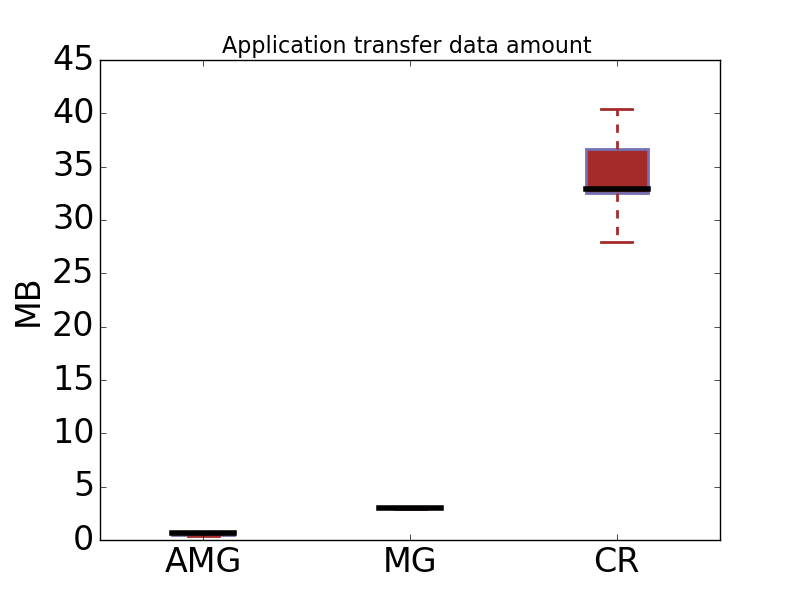
\includegraphics[width = 0.48\textwidth ]{data_amount}
%   \caption{Applications Data Transfer Amount. AMG has the least amount of data transfer, compared with MultiGrid and CrystalRouter.\NOTE{y axis in log?} }
%   \label{fig:3app-data-amount}
% \end{figure}
% 
% Figure \ref{fig:3app-data-amount} shows the data transfer amount of each MPI rank of three application. Based on this figure, we can tell that CrystalRouter is the most communication-intensive and AMG is the lest communication-intensive. 
% 
% 
% \subsection{Workload Analysis}
%  
% \begin{figure}[h!]
%   \centering
%   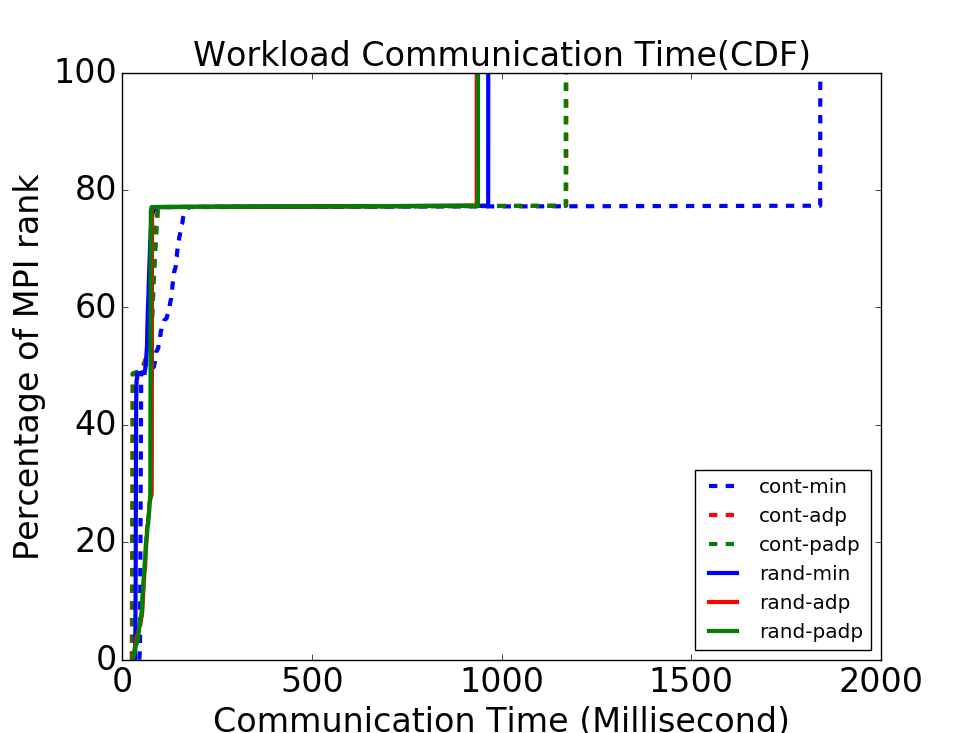
\includegraphics[width = 0.48\textwidth ]{wkld/wkld-commtime}
%   \caption{Time spent on communication by Workload I when 6 different placement and routing configurations are used. Random is better than contiguous in terms of improving communication efficiency. Communication time can be further reduced when (progressive) adaptive routing is used under both placement schemes. }
%   \label{fig:wkld-commtime}
% \end{figure}

\begin{table}[ht]
\begin{center}
\caption{Time spent on communication (MilliSecond) by Workload II when 6 different placement\&routing configuration in use.} 
\label{tab:wkld-commtime}
%\centering % Centers the table on the page, comment out to left-justify
\begin{tabular}{l c c c c c c }
\toprule % Top horizontal line
\toprule
&\multicolumn{6}{c}{Placement\&Routing Configuration} \\ % Amalgamating several columns into one cell is done using the \multicolumn command as seen on this line
\cmidrule(l){2-7}
	 & CM & CA & CPA & RM & RA & RPA \\ % Column names row
\midrule % In-table horizontal line
Runtime  &  1870 & 1250 & 1248 & 860 & 835 &830\\ % Content row 1

\midrule % In-table horizontal line
\bottomrule % Bottom horizontal line
\end{tabular}
\end{center}
\end{table}




The communication time spent by parallel workload \Rmnum{1} under different placement and routing configuration shown in Table \ref{tab:wkld-commtime}. The contiguous placement coupled with minimal routing results in highest communication time. Progressive adaptive and adaptive routing have comparable results when coupled with contiguous placement. The random placement results the comparable performance with any routing schemes and they all outperform the contiguous placement configurations.




\begin{figure*}[t!]
    \centering
    \begin{subfigure}[t]{0.32\textwidth}
        \centering
        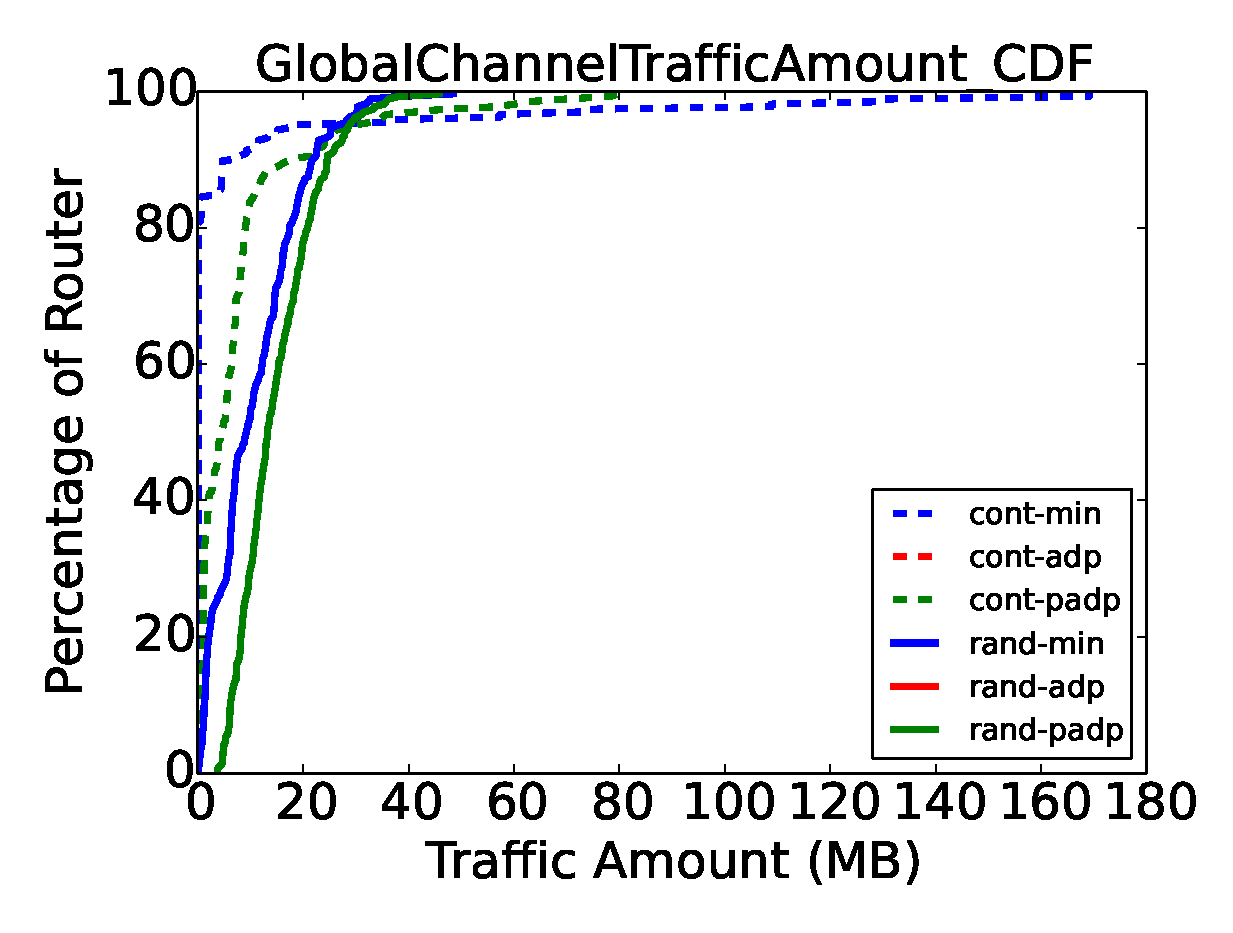
\includegraphics[height=1.8 in]{wkld/gc-traffic}
        \caption{Global Channel Traffic}
        \label{fig:global-channel-traffic}
    \end{subfigure}\hfill
    \hspace{1em}%
    \begin{subfigure}[t]{0.32\textwidth}
        \centering
        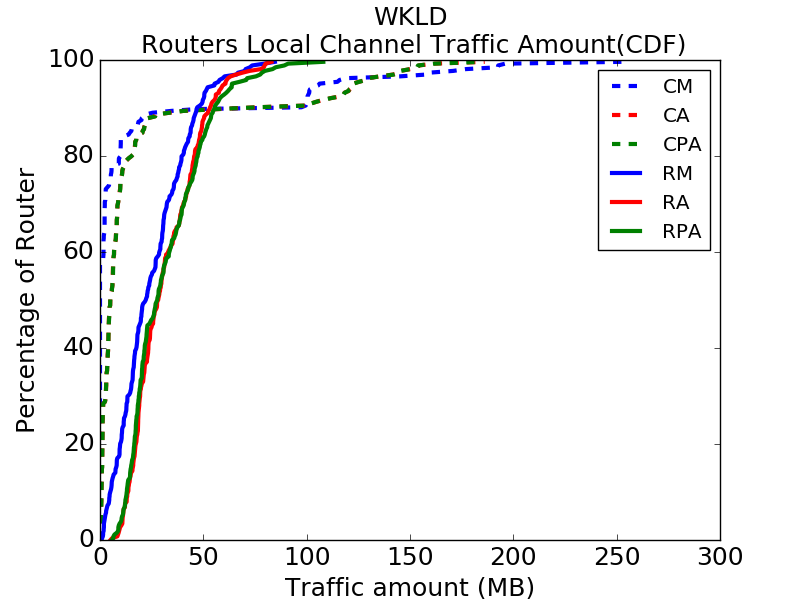
\includegraphics[height=1.8 in]{wkld/lc-traffic}
        \caption{Local Channel Traffic}
        \label{fig:local-channel-traffic}
    \end{subfigure}\hfill
    \hspace{1em}%
    \begin{subfigure}[t]{0.32\textwidth}
        \centering
        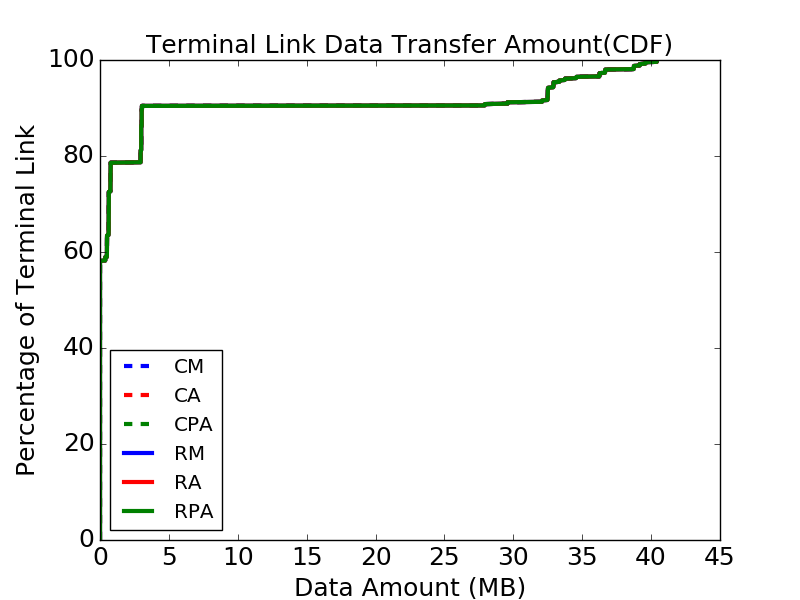
\includegraphics[height=1.8 in]{wkld/tl-traffic}
        \caption{Terminal Link Traffic}
        \label{fig:terminal-link-traffic}
    \end{subfigure}\\

    \centering   
    \begin{subfigure}[t]{0.32\textwidth}
        \centering
        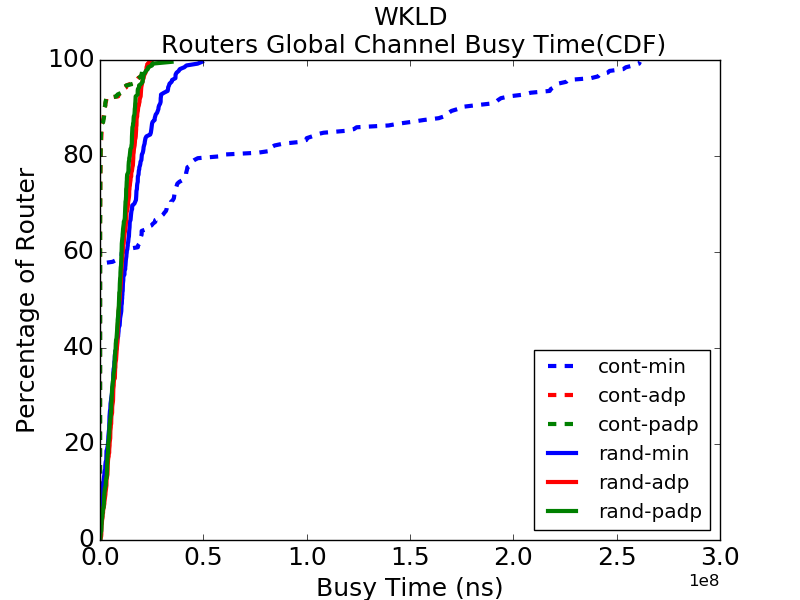
\includegraphics[height=1.8 in]{wkld/gc-stime}
        \caption{Global Channel Busy Time}
        \label{fig:global-channel-stime}
    \end{subfigure}\hfill
     \hspace{1em}%
    \begin{subfigure}[t]{0.32\textwidth}
        \centering
        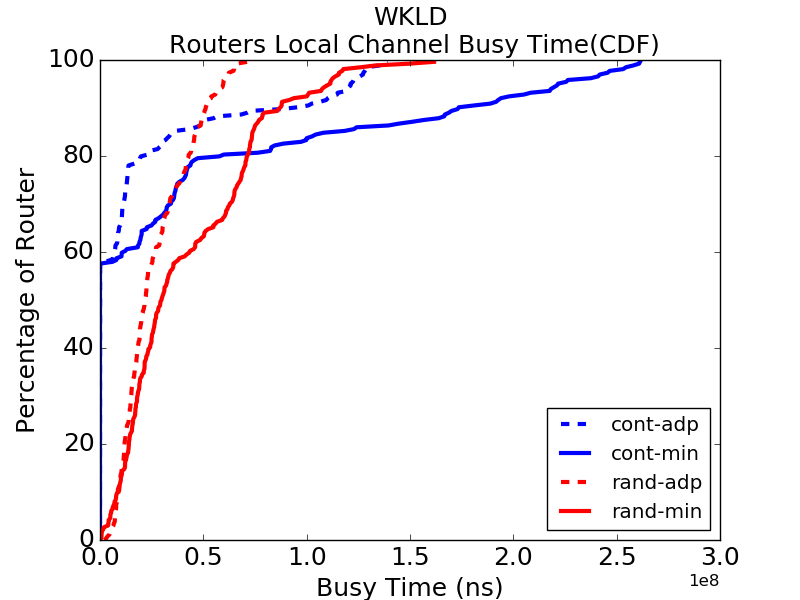
\includegraphics[height=1.8 in]{wkld/lc-stime}
        \caption{Local Channel Busy Time}
        \label{fig:local-channel-stime}
    \end{subfigure}\hfill
    \hspace{1em}%
    \begin{subfigure}[t]{0.32\textwidth}
        \centering
        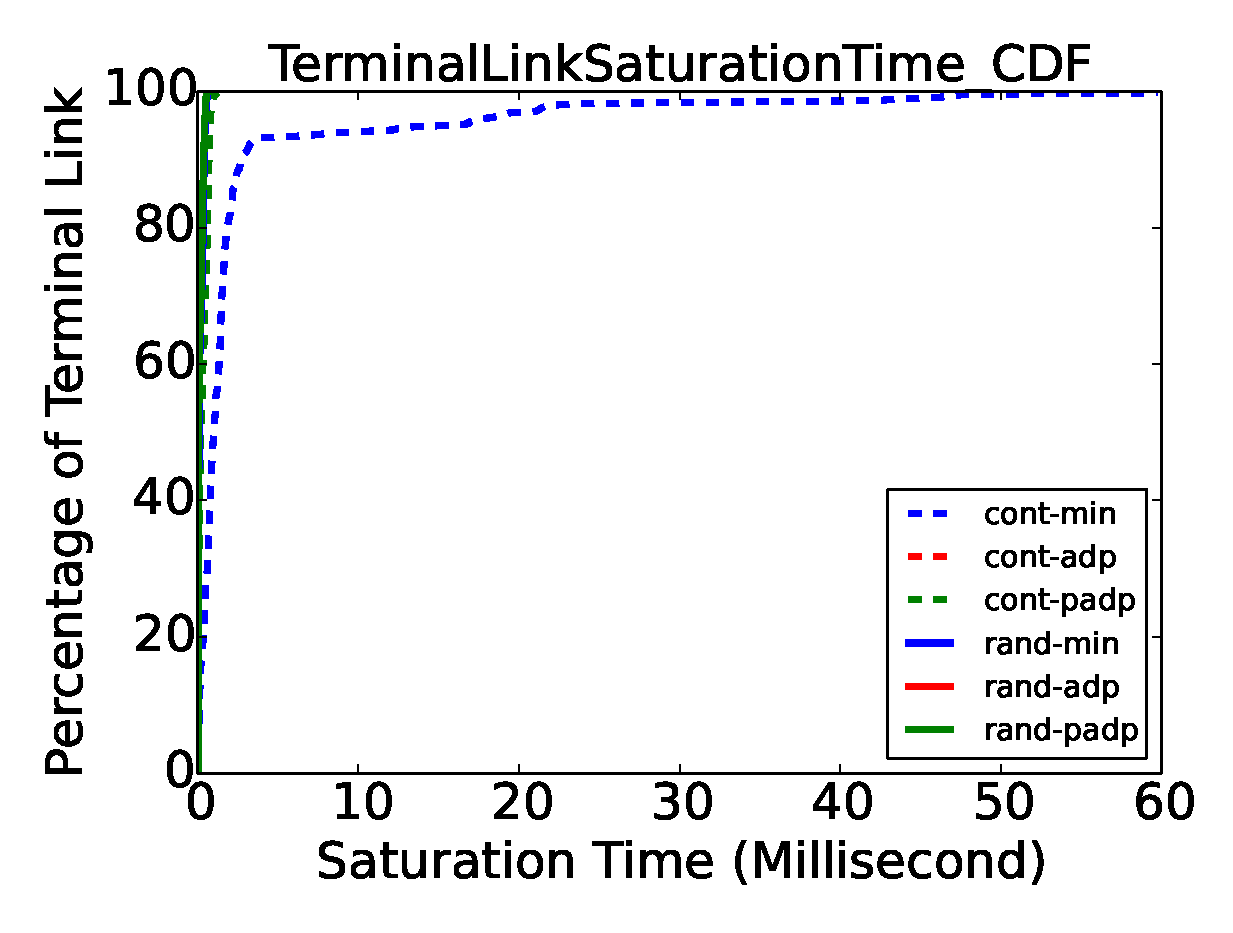
\includegraphics[height=1.8 in]{wkld/tl-stime}
        \caption{Terminal Link Busy Time}
        \label{fig:terminal-link-stime}
    \end{subfigure}%
   \caption{Traffic and saturated time of links in different level in the dragonfly network. The Workload \Rmnum{1} running under 6 different placement \& routing configuration.}
   \label{fig:wkld-network-traffic-stime}
\end{figure*}

Figure \ref{fig:wkld-network-traffic-stime} shows the amount of traffic go through terminal links, local channels and global channels, and the corresponding saturated time when the workload running on dragonfly network with 6 different placement and routing configurations 


%global link traffic and busy time explanation
When the workload is running with contiguous placement and minimal routing, all the MPI ranks are physically adjacent to each other, and the packets are routed through the shortest path between its source rank to destination rank. In this case, all the traffic are on the first half of the network (node id from 0 to $216+125+100-1=440$, group id from 0 to 13 ), causing local congestion and traffic load on some routers are extremely high, as shown the blue dash line in Figure \ref{fig:global-channel-traffic}. Thus the busy time of global channel is also the highest when contiguous placement coupled with minimal routing, as shown in Figure \ref{fig:global-channel-stime} the blue dash line. 

When contiguous placement is coupled with (progressive) adaptive routing, the local congestion on global channel will be greatly alleviated, as shown in Figure \ref{fig:global-channel-traffic} the red and green dash line. Since (progressive) adaptive routing are congestion aware, and be able to utilize the idle routers on the other part of the network. The busy time of global channel are also reduce by using contiguous placement coupled with either adaptive or progressive adaptive routing, as shown in Figure \ref{fig:global-channel-stime} the red and green dash line. 

Random placement can randomly allocate the MPI ranks to the physical nodes all over the network, thus prevent certain part of the network from being congested by traffic. Shown as the solid lines in Figure \ref{fig:global-channel-traffic}, the traffic go through global channels are uniformly distributed across all the routers in the network, thus no particular global channel will suffer high traffic burden. When the random placement coupled with minimal routing, the packets can avoid unnecessary intermediate forwarding as introduced by adaptive and progressive routing, which results in generating less traffic. That's why the blue solid line is lower than the red and green solid line. Since the random placement can uniformly distribute the workload traffic, there are no sudden surge of busy time of global channel over the network, shown as solid lines in Figure \ref{fig:global-channel-stime}.

%local channel traffic and busy time explanation

We can get the same observation from the local channel traffic (Figure \ref{fig:local-channel-traffic}) and busy time (Figure \ref{fig:local-channel-stime}). Contiguous placement coupled with minimal routing results in local congestion, thus highest traffic amount on the local channel of certain routers. Even with adaptive or progressive adaptive routing, the local congestion caused by grouping MPI rank on adjacent nodes in contiguous placement can not be eliminated. The random placement can reduce the congestion on local channel for allocating MPI ranks to random selected nodes. 

%terminal link traffic and busy time explanation
The distribution of traffic go through terminal links stay unchanged no matter which placement \& routing configuration in use, as shown in Figure \ref{fig:terminal-link-traffic}. This is because only the location of each MPI rank in the network will be changed in different placement schemes, and the routing won't have effect the terminal link, so the traffic between compute node and the router won't change. Due to the traffic changes on global and local channels, the busy time of terminal links will experience variability when different routing schemes in use, as shown in Figure \ref{fig:terminal-link-stime}. 


 
% \NOTE{The take-home message} from Figure \ref{fig:wkld-network-stime} and \ref{fig:wkld-network-traffic}. 

Contiguous placement allocates MPI ranks to physical nodes that are adjacent to each other, which confines the workload traffic to some local area when coupled with minimal routing. This may result in local congestion and unbalanced network utilization. Contiguous placement coupled with minimal routing always leads to the extreme high traffic amount for some routers , and thus longest busy time.

Random placement allocates MPI ranks to a set of randomly selected nodes all over the system, uniformly distributes workload traffic and avoids local congestion. When random placement is coupled with minimal routing, the packets will take the shortest path from source router to the destination router without routing to any intermediate routers, this will prevent the routing from generating extra traffic. When random placement is coupled with adaptive or progressive adaptive routing, the possibility of any congestion will be further reduced at the cost of extra intermediate traffic. 

The random job placement coupled with either minimal or adaptive routing can reach hot-spots free and load-balanced by distributing the workload traffic over the network. The workload performance get greatly improved with this configuration. However, when we isolated individual application from the workload, we unveil the fact that not every application can benefit from random job placement. 


% Start from here, we present the individual application analysis.
\subsection{Individual Application Analysis}

\begin{figure*}[t!]
    \centering
    \begin{subfigure}[t]{0.32\textwidth}
        \centering
        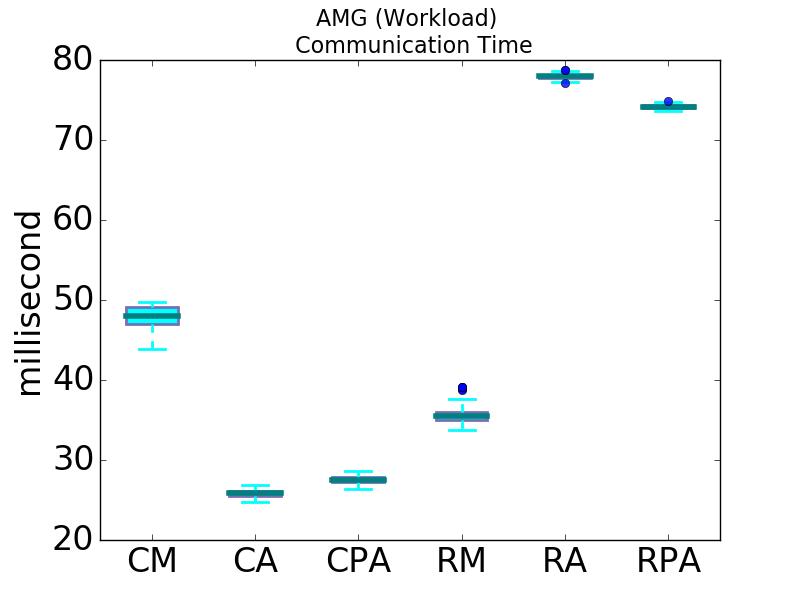
\includegraphics[height=1.5 in]{amg/commtime}
        \caption{AMG Communication Time}
        \label{fig:amg-commtime}
    \end{subfigure}%
    \hspace{1em}%
    \begin{subfigure}[t]{0.32\textwidth}
        \centering
        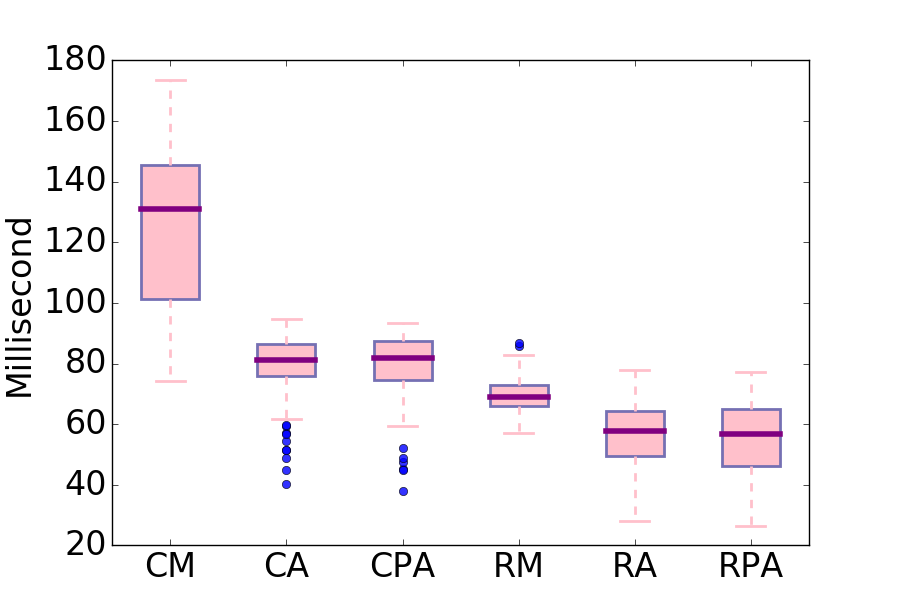
\includegraphics[height=1.5 in]{mg/commtime}
        \caption{MG Communication Time}
        \label{fig:mg-commtime}
    \end{subfigure}%
    \begin{subfigure}[t]{0.32\textwidth}
        \centering
        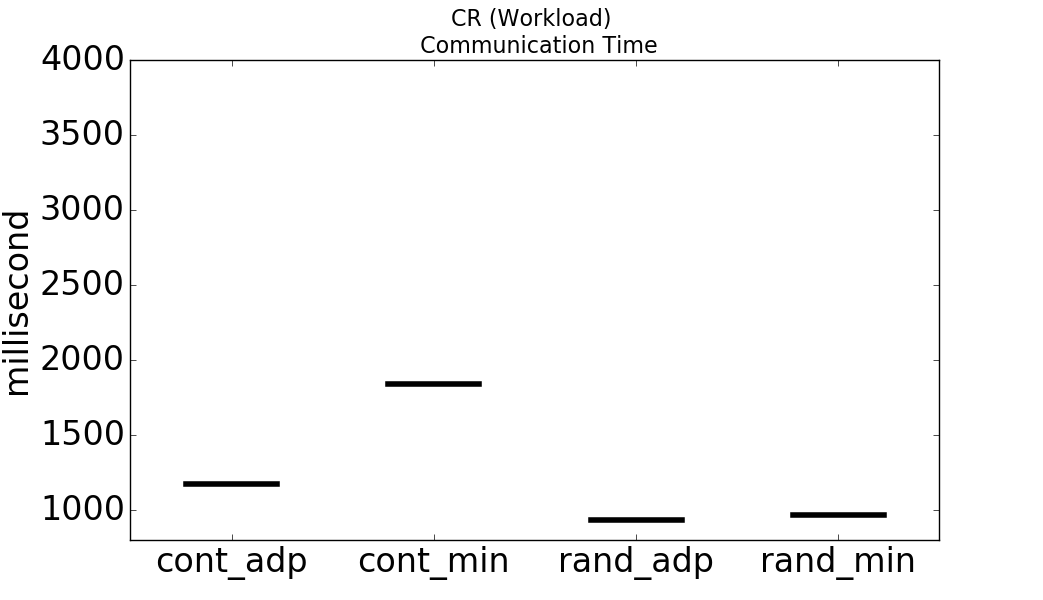
\includegraphics[height=1.5 in]{cr/commtime}
        \caption{CR Communication Time}
        \label{fig:cr-commtime}
    \end{subfigure}%
   \caption{Application communication time. Three applications running concurrently on dragonfly network with different placement and routing configurations. Random placement and adaptive routing can improve MG and CR communication, however, AMG's communication time is greatly prolonged.}
   \label{fig:apps-commtime}
\end{figure*}

Figure \ref{fig:apps-commtime} shows the communication time of three applications running concurrently under 6 different placement and routing configurations listed in Table\ref{tab: placement routing configs}.

As shown in Figure \ref{fig:mg-commtime}, \ref{fig:cr-commtime}, MG and CR suffer the longest communication time when running with contiguous placement \& minimal routing (CM). When contiguous placement coupled with adaptive or progressive adaptive routing (CA, CPA), both MultiGrid and CrystalRouter will get great improvement, their communication time reduce a lot. Random placement will further reduce the communication time of MultiGrid and CrystalRouter, and reach the best performance when coupled with (progressive) adaptive routing (RPA, RA). Both MultiGrid and CrystalRouter shows the same trend as the workload when running under different placement \& routing configurations. 

AMG is quite an exception. As shown in Figure \ref{fig:amg-commtime}, the communication time of AMG is skyrocketing when it running under random placement coupled with (progressive) adaptive routing (RPA, RA). The contiguous placement coupled with (progressive) adaptive routing can reach the best performance for AMG. The performance of AMG running under contiguous placement coupled with minimal routing (CM) is no better than random coupled with minimal routing (RM), but still much better than random with (progressive) adaptive routing (RPA, RA). 



\begin{figure*}[t]
    \centering
    \begin{subfigure}[t]{0.32\textwidth}
        \centering
        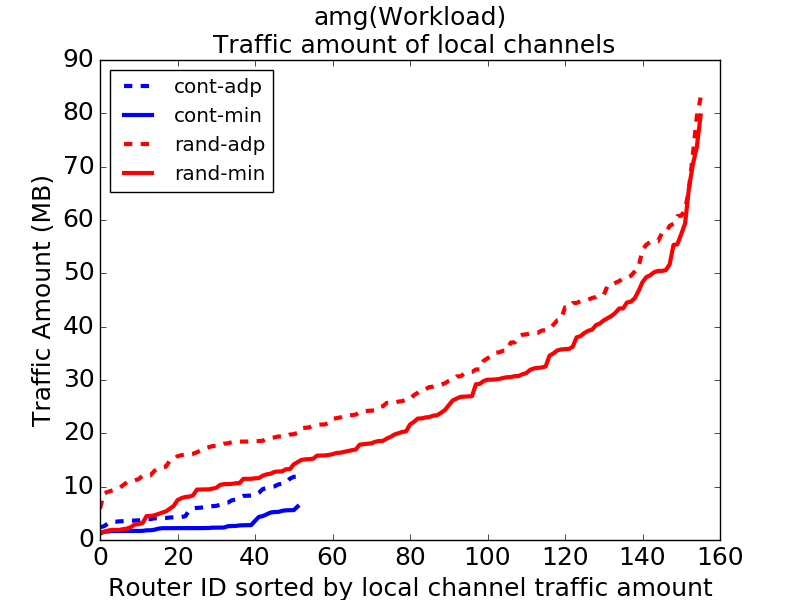
\includegraphics[height=1.8 in]{amg/lc-traffic}
        \caption{AMG Local Channel Traffic}
        \label{fig:amg-lc-traffic}
    \end{subfigure}\hfill
    \hspace{1em}%
    \begin{subfigure}[t]{0.32\textwidth}
        \centering
        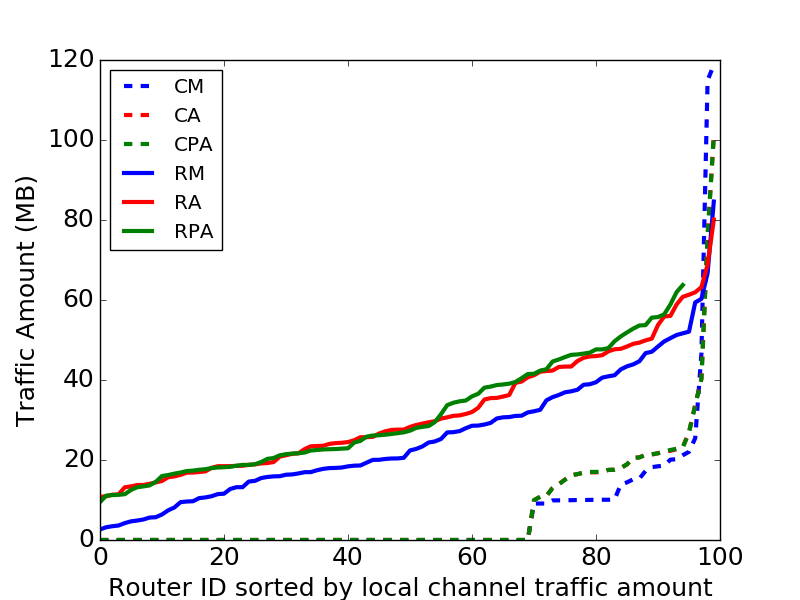
\includegraphics[height=1.8 in]{mg/lc-traffic}
        \caption{MG Local Channel Traffic}
        \label{fig:mg-lc-traffic}
    \end{subfigure}\hfill
    \begin{subfigure}[t]{0.32\textwidth}
        \centering
        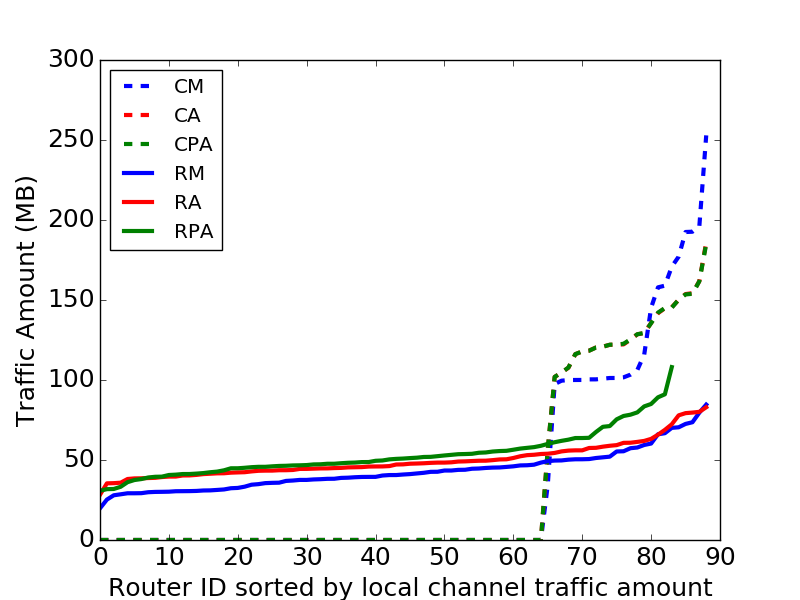
\includegraphics[height=1.8 in]{cr/lc-traffic}
        \caption{CR Local Channel Traffic}
        \label{fig:cr-lc-traffic}
    \end{subfigure}\\

    \centering
    \begin{subfigure}[t]{0.32\textwidth}
        \centering
        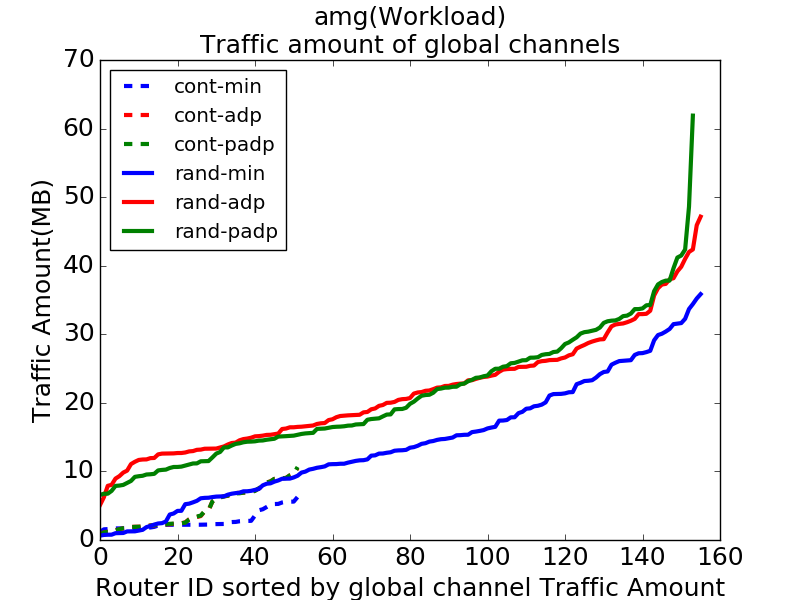
\includegraphics[height=1.8 in]{amg/gc-traffic}
        \caption{AMG Global Channel Traffic}
        \label{fig:amg-gc-traffic}
    \end{subfigure}\hfill
    \hspace{1em}%
    \begin{subfigure}[t]{0.32\textwidth}
        \centering
        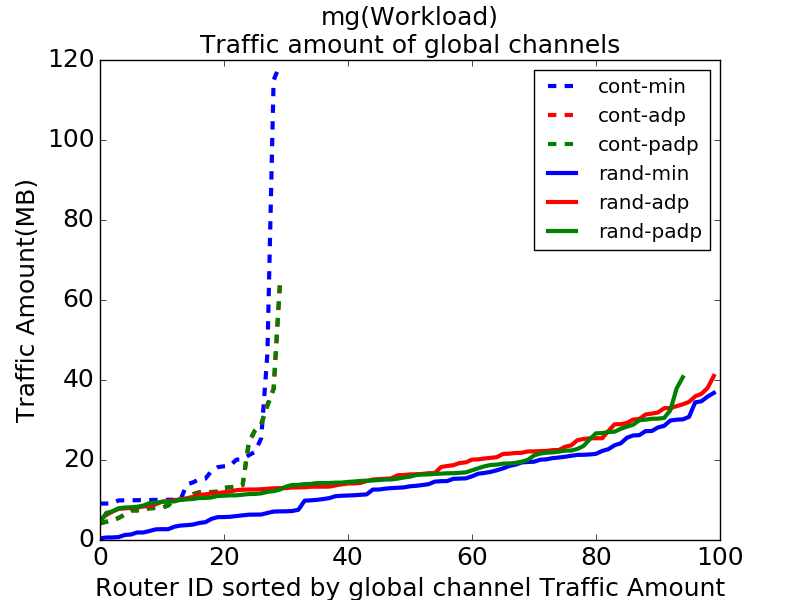
\includegraphics[height=1.8 in]{mg/gc-traffic}
        \caption{MG Global Channel Traffic}
        \label{fig:mg-gc-traffic}
    \end{subfigure}\hfill
    \begin{subfigure}[t]{0.32\textwidth}
        \centering
        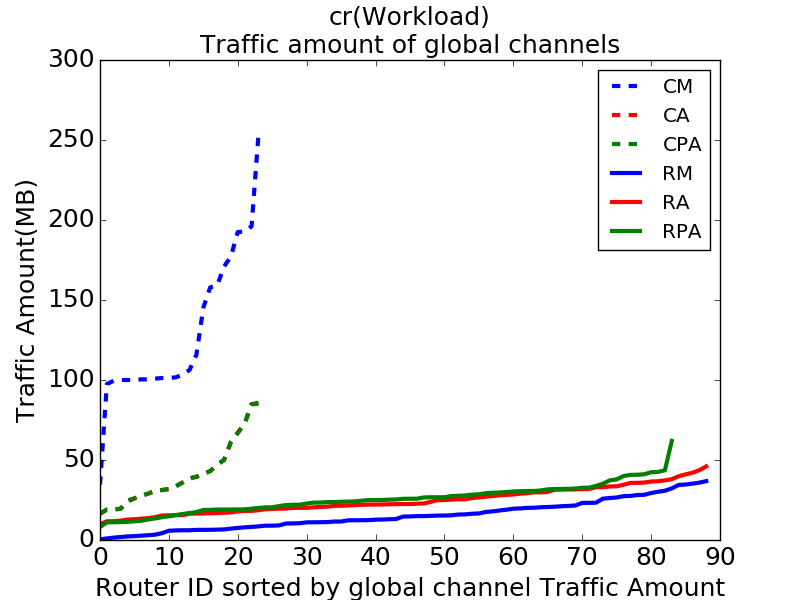
\includegraphics[height=1.8 in]{cr/gc-traffic}
        \caption{CR Global Channel Traffic}
        \label{fig:cr-gc-traffic}
    \end{subfigure}%
   \caption{The traffic go through the local and global channels of routers that belongs to specific application.}
   \label{fig:3app-lc-gc-traffic}
\end{figure*}





% Show the evidence from network level, explain why AMG is different. 
We look into network level to identify the culprit behind AMG's abnormal behavior with random placement \& adaptive routing. By identifying the terminal nodes each MPI rank resides on and routers that each application's traffic go through, we can see that the traffic go through the routers that belongs to AMG is skyrocketing when random placement \& adaptive routing is in use, shown in Figure \ref{fig:amg-lc-traffic} and Figure \ref{fig:amg-gc-traffic}. Adaptive routing will redirect the traffic of other applications to go through the routers belongs to AMG, and increase the traffic burden on those routers, thus slow down the communication of AMG.

No router will be shared between applications under contiguous placement. A set of successive groups will be allocated to each application under contiguous placement scheme. When contiguous placement coupled with minimal routing, application will be free of interference from its concurrently running peers. However, application communication traffic will be confined within their allocated routers, thus local congestion is very likely to happen depends on application communication intensity. As the lest communication intensive application in the workload, AMG can benefit from contiguous placement. Under contiguous placement, the traffic go through the local and global channels of the routers that belongs to AMG is significantly lower than random placement, shown in Figure \ref{fig:amg-lc-traffic}, \ref{fig:amg-gc-traffic}. 

MultiGrid and CrystalRouter are more communication intensive compared with AMG. They will suffer great amount local traffic in both local and global channels when contiguous placement is used, shown as the dash line in Figure \ref{fig:mg-lc-traffic}, \ref{fig:mg-gc-traffic} and Figure \ref{fig:cr-lc-traffic}, \ref{fig:cr-gc-traffic}. On the other hand, the random placement scheme can uniformly distribute their traffic all over the network by allocating randomly selected nodes to each MPI rank, shown as the solid lines in Figure \ref{fig:mg-lc-traffic}, \ref{fig:mg-gc-traffic} and Figure \ref{fig:cr-lc-traffic}, \ref{fig:cr-gc-traffic}.



So far we know that the reason for AMG being the only victim from random placement \& adaptive routing is due to its relatively small amount of data transfer, that make it the least communication-intensive application in the workload.

\subsection{Key Findings}
We can get the following key findings from the detailed analysis of three applications. 

\emph{Random placement \& adaptive routing is quite efficient for orchestrate the traffic load in the network by uniformly distributing the workload traffic all over the network. However, application like AMG will be impaired in this orchestration. The routers through which the less communication-intensive application traffic used to route, now have more traffic go through them. These extra traffic are from other communication-intensive applications. Beneath the facade of harmony, less communication-intensive application are ``bullied" by their concurrently running communication-intensive peers in the workload. }

\emph{Random placement \& adaptive routing can not guarantee QoS for each application in the workload. In order to reach load-balanced and hot-spots free, the traffic from congested routers will be redirected to other less busy routers. This will indulge the ``bully" that communication-intensive applications impose to their less intensive peers.}

\emph{Contiguous placement \& minimal routing guarantee a consistent performance of each application. Although, contiguous placement and minimal routing usually results in local congestion and unbalanced network utilization, it can reduce the interference between concurrently running applications, thus prevent less communication-intensive application from being ``bullied" by its communication-intensive peers.}

We have tried three different congestion sensing schemes that used in adaptive routing\cite{won-prog-adaptive}, although there are some variations between the results, none of the congestion sensing scheme can prevent the ``bully" from happening.

\section{Parallel Workload \Rmnum{2 }}
\label{sec:workload-2}


In order to prove that AMG being bullied only because it is less communication-intensive than its concurrently running peers, we generate a synthetic application, sAMG, which are same the with AMG's original traces in every aspect expect that the data transfer amount 100x greater than AMG. We run the new workload that consists of sAMG, MultiGrid and CrystalRouter on the same dragonfly network with the same placement \& routing configurations. As shown in Table \ref{tab:apps-detail}, sAMG become the most communication-intensive application in the new workload. 

\subsection{Workload Analysis}


\begin{table}[ht]
\begin{center}
\caption{Time spent on communication (MilliSecond) by Workload II when 6 different placement\&routing configuration in use.} 
\label{tab:syn-wkld-commtime}
%\centering % Centers the table on the page, comment out to left-justify
\begin{tabular}{l c c c c c c }
\toprule % Top horizontal line
\toprule
&\multicolumn{6}{c}{Placement\&Routing Configuration} \\ % Amalgamating several columns into one cell is done using the \multicolumn command as seen on this line
\cmidrule(l){2-7}
	 & CM & CA & CPA & RM & RA & RPA \\ % Column names row
\midrule % In-table horizontal line
Runtime  &  6123 & 3231 & 3725 & 2544 & 3701 & 3228 \\ % Content row 1

\midrule % In-table horizontal line
\bottomrule % Bottom horizontal line
\end{tabular}
\end{center}
\end{table}


The communication time spent by parallel workload \Rmnum{2} under different placement \& routing configurations shown in Table \ref{tab:syn-wkld-commtime}. As the overall traffic increased in the workload(due to sAMG), the time spent on communication under each configuration also increases. But the performance of each configuration still keep the same trend as parallel workload \Rmnum{1}. The contiguous placement coupled with minimal routing results in highest communication time. The random placement coupled with minimal routing is the most efficient. Progressive adaptive routing is better than adaptive routing when random placement is in use. And they have comparable results when coupled contiguous placement. 


Figure \ref{fig:synwkld-network-traffic-stime} show the network status when Workload \Rmnum{2} running under different placement \& routing configurations. Contiguous placement coupled with minimal routing result in most traffic go through certain local and global channel, thus the longest  communication time for terminal link, local and global channel. When coupled with (progressive) adaptive routing, the local congestion can get alleviated in contiguous placement. The random placement reach the comparable performance with any routing schemes in terms of both traffic and busy time. They are better than contiguous \& minimal configuration, but not too much improvement against contiguous\&(progressive) adaptive configuration.



\begin{figure*}[t]
    \centering
    \begin{subfigure}[t]{0.32\textwidth}
        \centering
        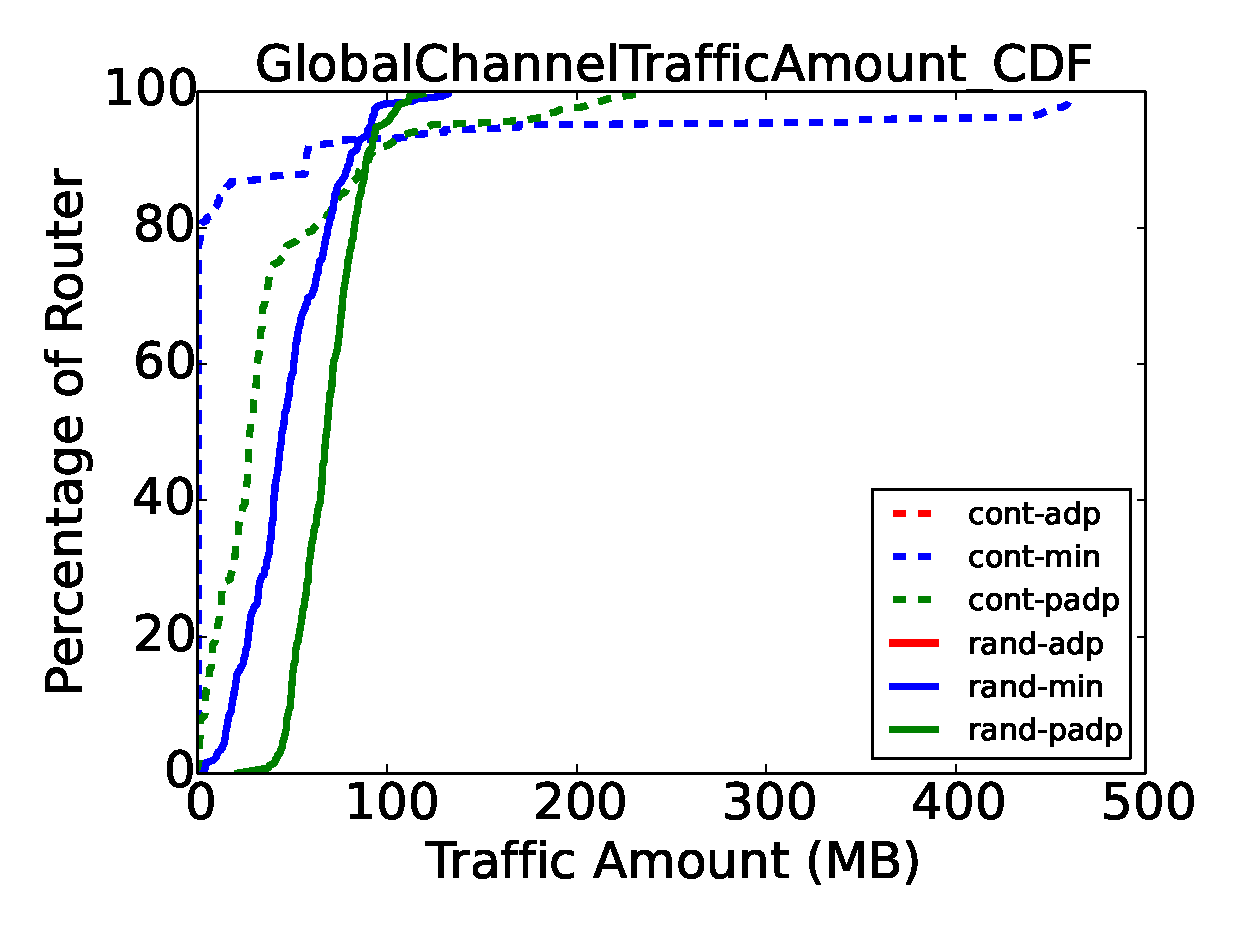
\includegraphics[height=1.8 in]{syn-wkld/gc-traffic}
        \caption{Global Channel Traffic}
        \label{fig:synwkld-global-channel-traffic}
    \end{subfigure}\hfill
    \hspace{1em}%
    \begin{subfigure}[t]{0.32\textwidth}
        \centering
        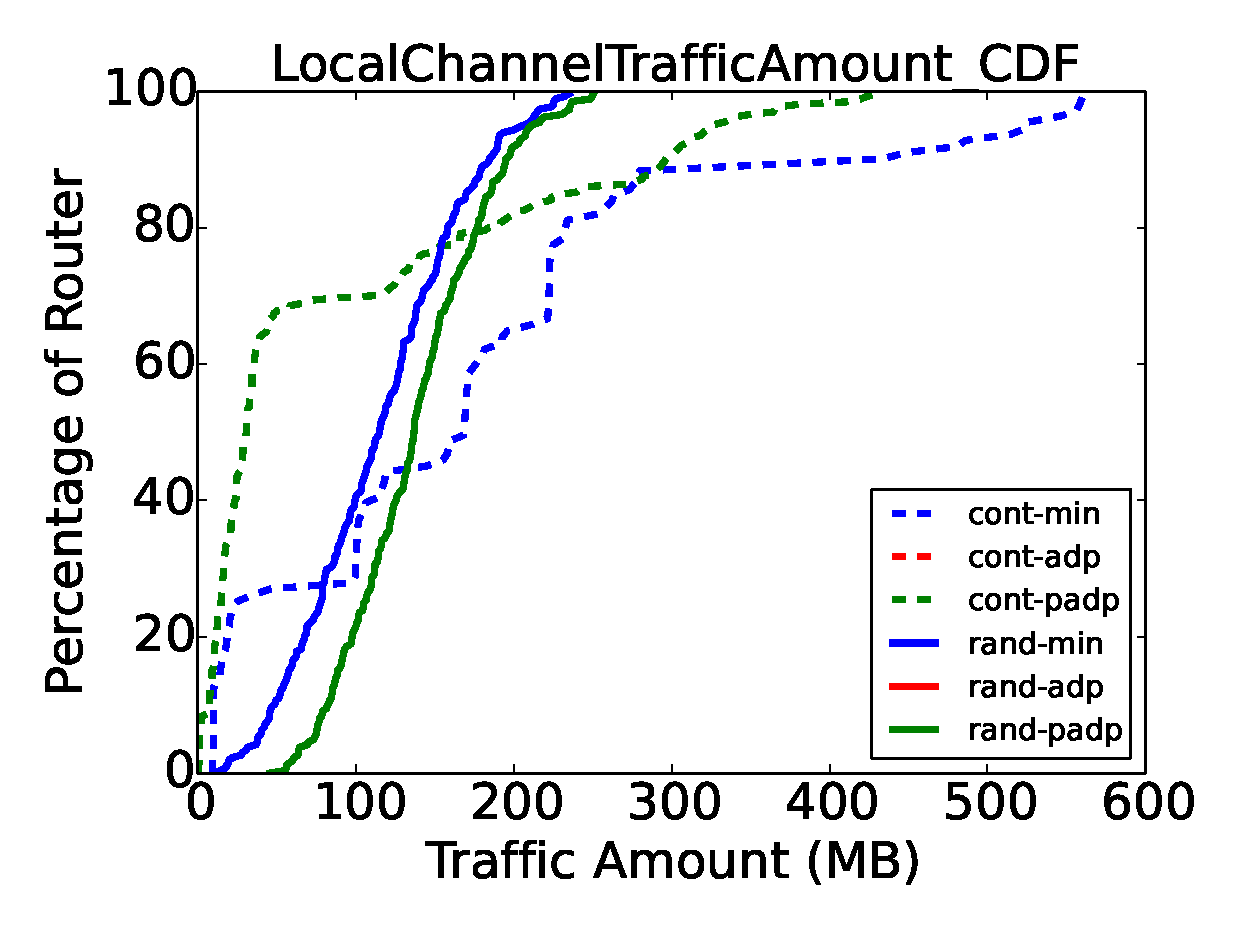
\includegraphics[height=1.8 in]{syn-wkld/lc-traffic}
        \caption{Local Channel Traffic}
        \label{fig:synwkld-local-channel-traffic}
    \end{subfigure}\hfill
    \hspace{1em}%
    \begin{subfigure}[t]{0.32\textwidth}
        \centering
        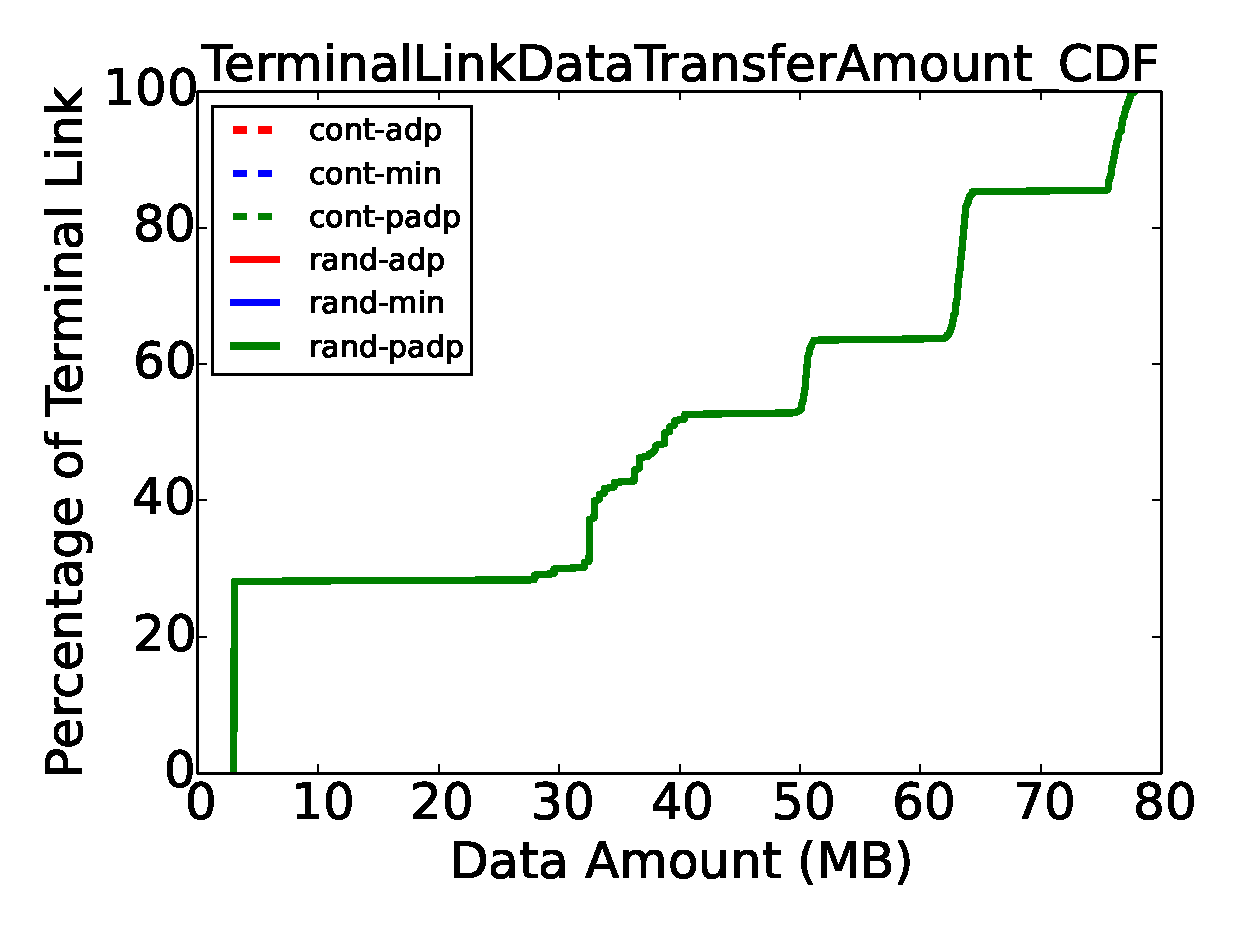
\includegraphics[height=1.8 in]{syn-wkld/tl-traffic}
        \caption{Terminal Link Traffic}
        \label{fig:synwkld-terminal-link-traffic}
    \end{subfigure}\\

    \begin{subfigure}[t]{0.32\textwidth}
        \centering
        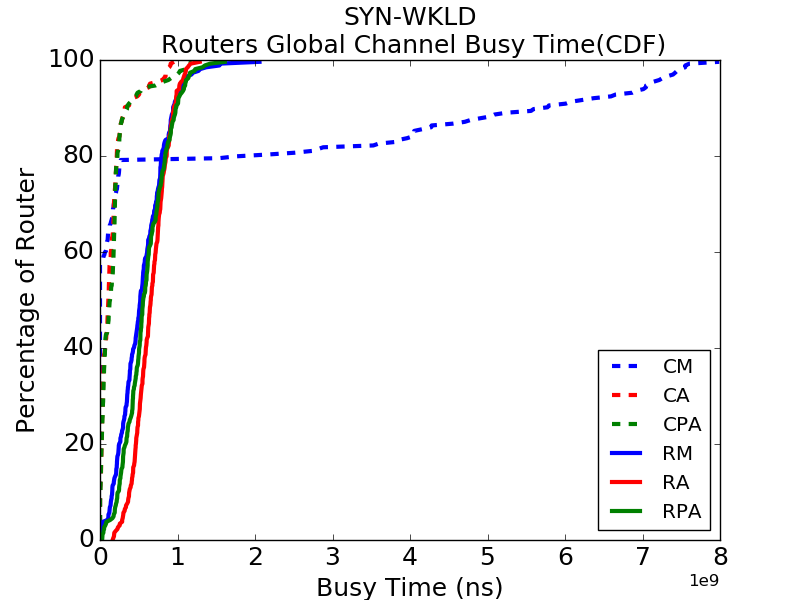
\includegraphics[height=1.8 in]{syn-wkld/gc-btime}
        \caption{Global Channel Busy Time}
        \label{fig:synwkld-global-channel-stime}
    \end{subfigure}\hfill
     \hspace{1em}%
    \begin{subfigure}[t]{0.32\textwidth}
        \centering
        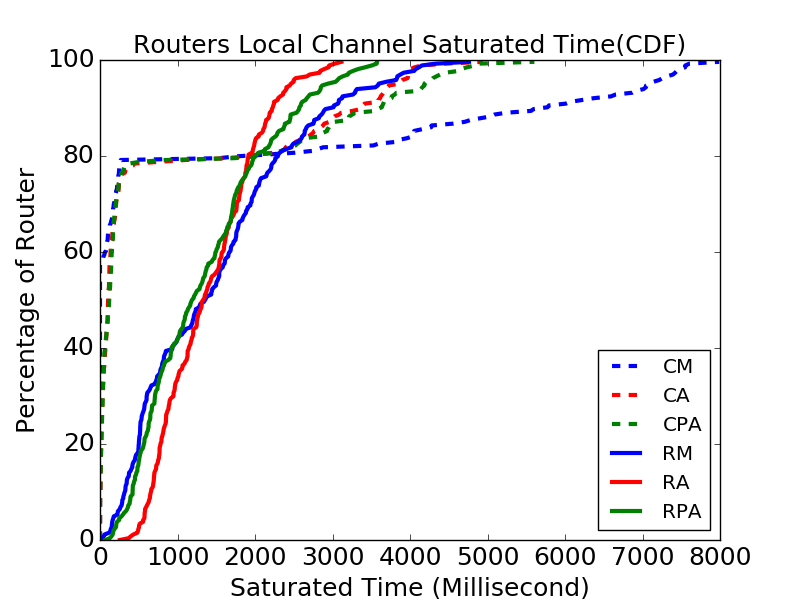
\includegraphics[height=1.8 in]{syn-wkld/lc-btime}
        \caption{Local Channel Busy Time}
        \label{fig:synwkld-local-channel-stime}
    \end{subfigure}\hfill
    \hspace{1em}%
    \begin{subfigure}[t]{0.32\textwidth}
        \centering
        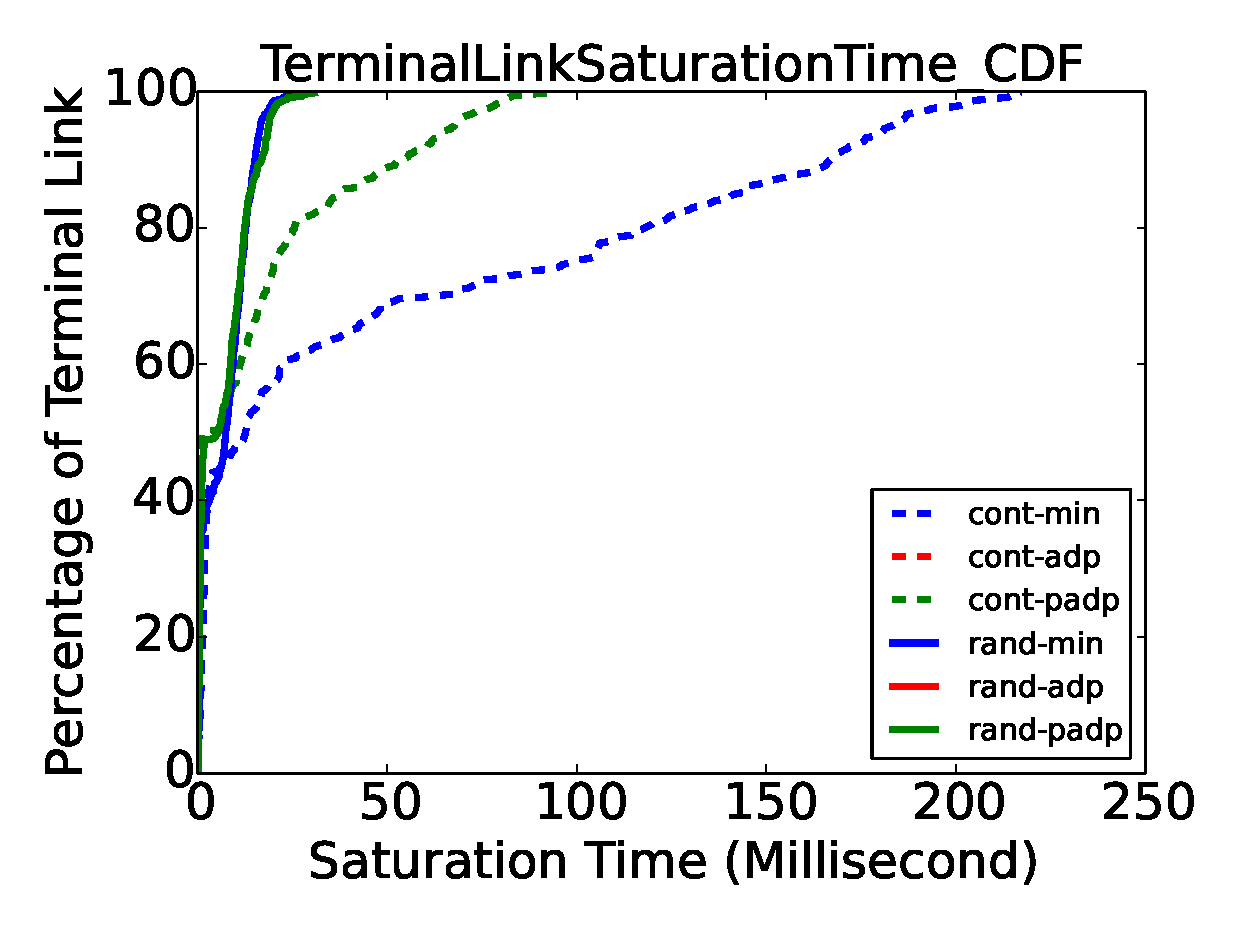
\includegraphics[height=1.8 in]{syn-wkld/tl-btime}
        \caption{Terminal Link Busy Time}
        \label{fig:synwkld-terminal-link-stime}
    \end{subfigure}%
   \caption{Traffic and Saturated Time of different level of links in the dragonfly network. The Workload \Rmnum{2} running under 6 different placement \& routing configuration.}
   \label{fig:synwkld-network-traffic-stime}
\end{figure*}

\subsection{Individual Application Analysis}

The communication time of each application shown in Figure \ref{fig:syn-apps-commtime}. The ``bully" become the ``bullyee". The less communication-intensive applications in Workload \Rmnum{2} are  MultiGrid and CrystalRouter.  When random placement coupled with (progressive) adaptive routing is used, MultiGrid and CrystalRouter suffer prolonged communication time, shown in Figure \ref{fig:syn-mg-commtime}, \ref{fig:syn-cr-commtime}. sAMG on the other hand benefit from random placement, shown in Figure \ref{fig:syn-samg-commtime}. 

Contiguous placement coupled with minimal routing prevent applications from sharing network resource, and confine application communication traffic to the routers assigned to each application. This can guarantee the performance of less communication intensive applications like MultiGrid and CrystalRouter, and make the communication intensive application like sAMG severely deteriorate. 


\begin{figure*}[t!]
    \centering
    \begin{subfigure}[t]{0.32\textwidth}
        \centering
        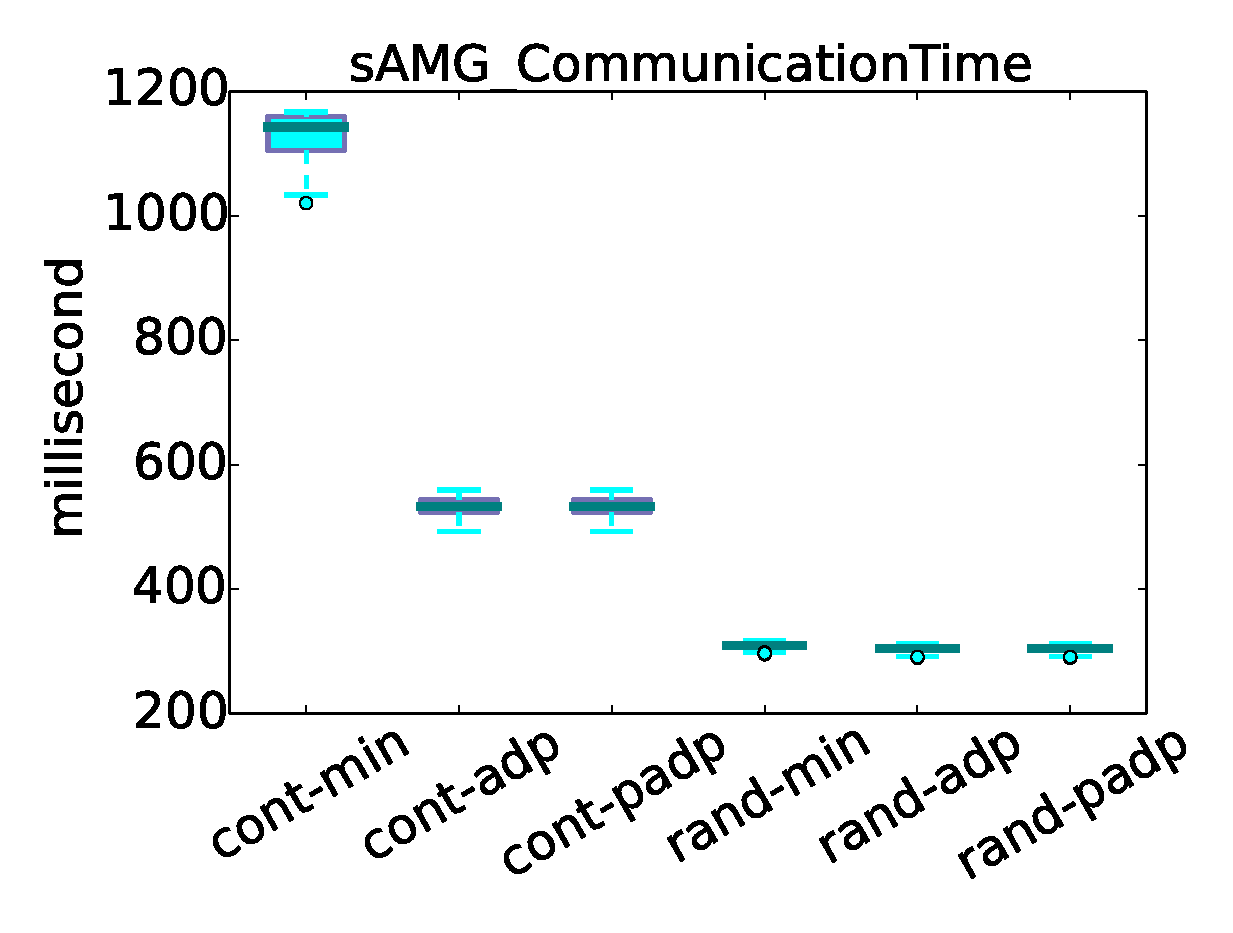
\includegraphics[height=1.5 in]{syn-wkld/amg10/commtime}
        \caption{sAMG Communication Time}
        \label{fig:syn-samg-commtime}
    \end{subfigure}%
    \hspace{1em}%
    \begin{subfigure}[t]{0.32\textwidth}
        \centering
        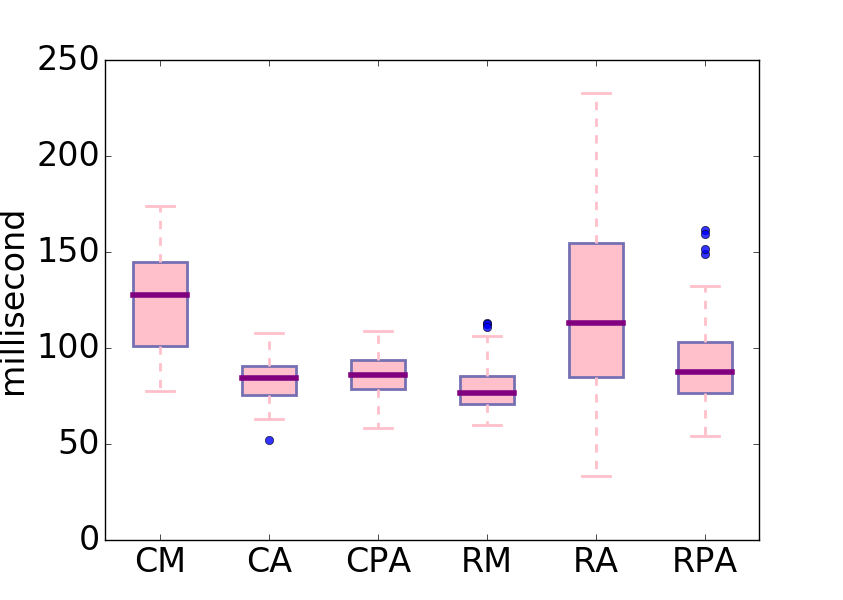
\includegraphics[height=1.5 in]{syn-wkld/mg/commtime}
        \caption{MG Communication Time}
        \label{fig:syn-mg-commtime}
    \end{subfigure}%
    \begin{subfigure}[t]{0.32\textwidth}
        \centering
        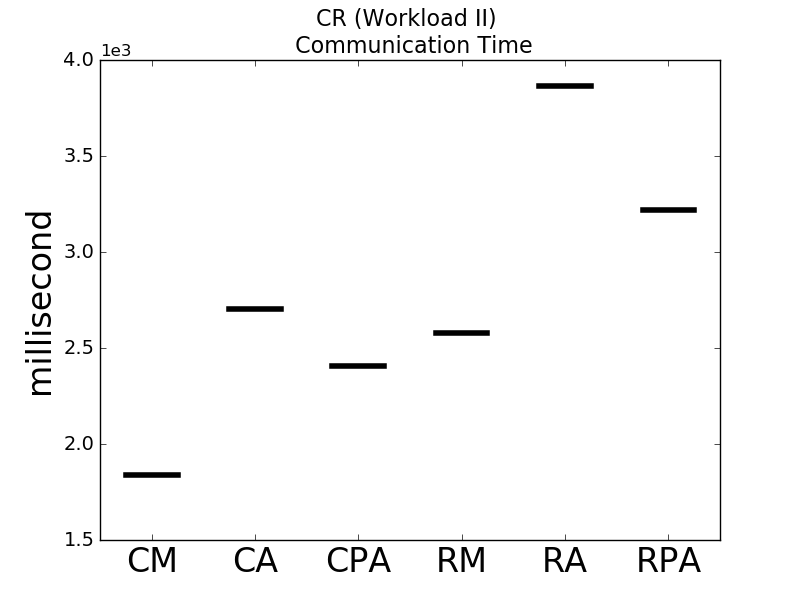
\includegraphics[height=1.5 in]{syn-wkld/cr/commtime}
        \caption{CR Communication Time}
        \label{fig:syn-cr-commtime}
    \end{subfigure}%
   \caption{Application communication time. Three applications running concurrently on dragonfly network with different placement and routing configurations. Random placement and adaptive routing can improves AMG's communication time. MG and CR communication time are prolonged with random placement and adaptive routing.}
   \label{fig:syn-apps-commtime}
\end{figure*}

% explain the network status of sAMG, MG and CR
We look into the network level to scrutinize the traffic go through the routers belongs to each application. 
Figure \ref{fig:syn-samg-lc-traffic}, \ref{fig:syn-samg-gc-traffic} shows the traffic go through the local and global channels of the routers that belongs to sAMG when different placement \& routing configuration in use. The traffic is skyrocketing in both local and global channels when contiguous placement coupled with minimal routing. The contiguous placement make all the MPI ranks of sAMG reside on a set of nodes in the groups that adjacent to each other and minimal routing confines the traffic in those groups, results in severe local congestion. When adaptive routing is used, the local congestion will be alleviated in both local and global channels, as some traffic will be redirected to other part of the network. Random placement scheme can further reduce the traffic burden on local and global channels by assigning each MPI rank of sAMG with randomly select nodes, thus uniformly distribute sAMG traffic over the network. 

MultiGrid become a victim of sAMG's bully when running under random placement. The traffic go through the local and global channels of the routers that belongs to MultiGrid are shown in Figure \ref{fig:syn-mg-lc-traffic}, \ref{fig:syn-mg-gc-traffic}. Although contiguous placement allocates all the MPI ranks in set of nodes in adjacent groups, causing possible local congestion, it will stop MultiGrid's routers being shared by the traffic from its communication-intensive peer, sAMG. As random placement is used, the traffic go through both local and global channels are greatly increased. 

CrystalRouter has more traffic than MultiGrid. The random placement won't redirect much traffic from other applications to the routers belongs to CrystalRouter, compared with contiguous placement, as shown in Figure \ref{fig:syn-cr-lc-traffic}, \ref{fig:syn-cr-gc-traffic}.



\begin{figure*}[t]
    \centering
    \begin{subfigure}[t]{0.32\textwidth}
        \centering
        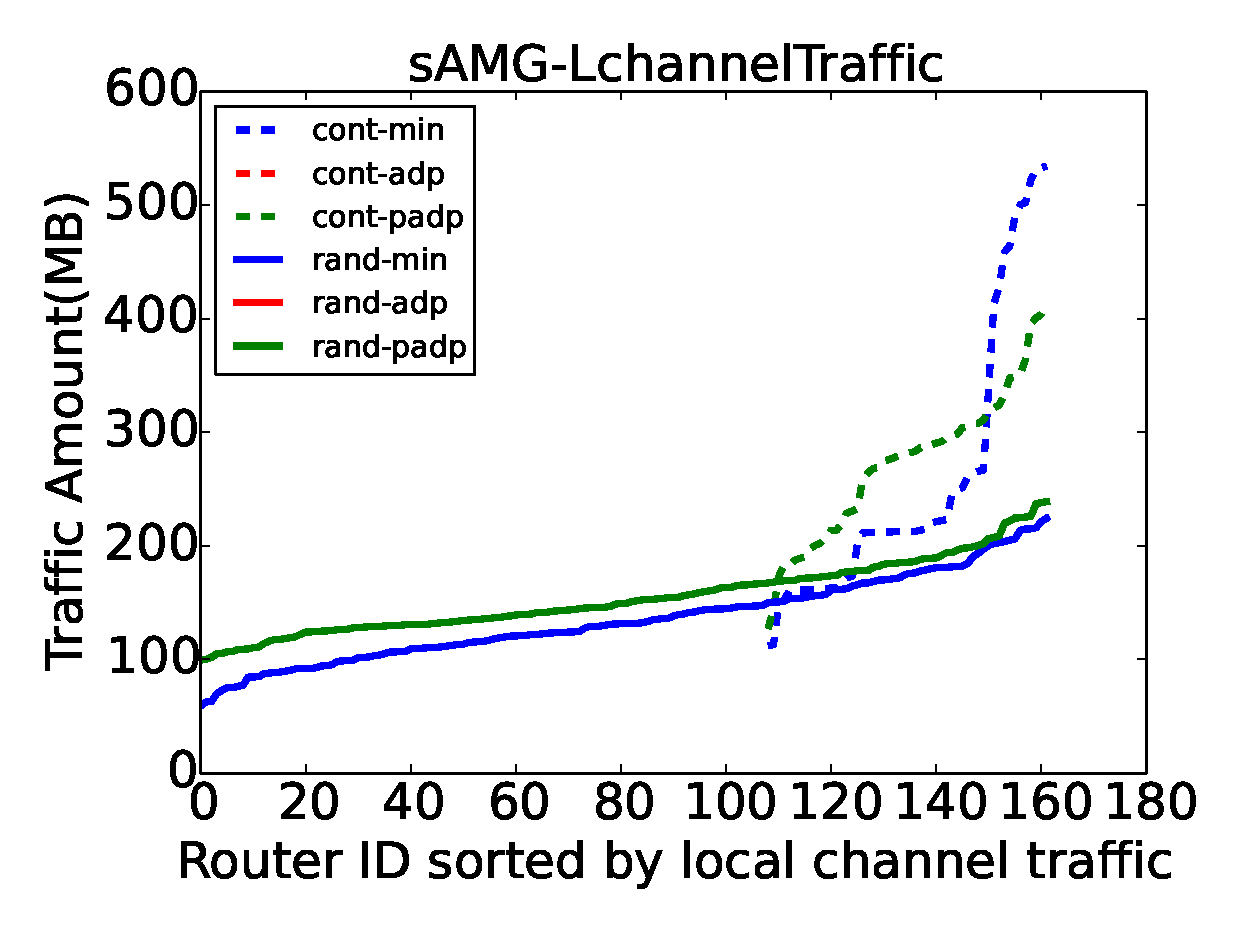
\includegraphics[height=1.5 in]{syn-wkld/amg10/lc-traffic}
        \caption{sAMG Local Channel Traffic}
        \label{fig:syn-samg-lc-traffic}
    \end{subfigure}\hfill
    \hspace{1em}%
    \begin{subfigure}[t]{0.32\textwidth}
        \centering
        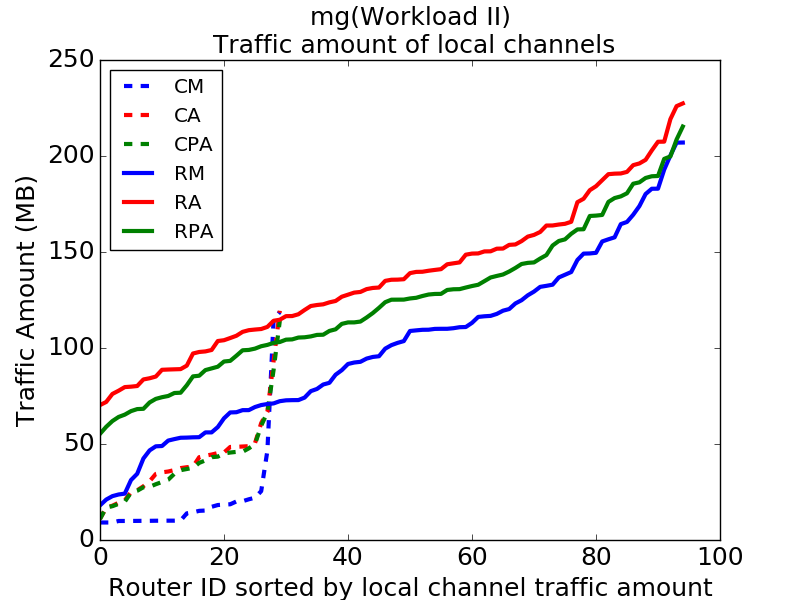
\includegraphics[height=1.5 in]{syn-wkld/mg/lc-traffic}
        \caption{MG Local Channel Traffic}
        \label{fig:syn-mg-lc-traffic}
    \end{subfigure}\hfill
    \begin{subfigure}[t]{0.32\textwidth}
        \centering
        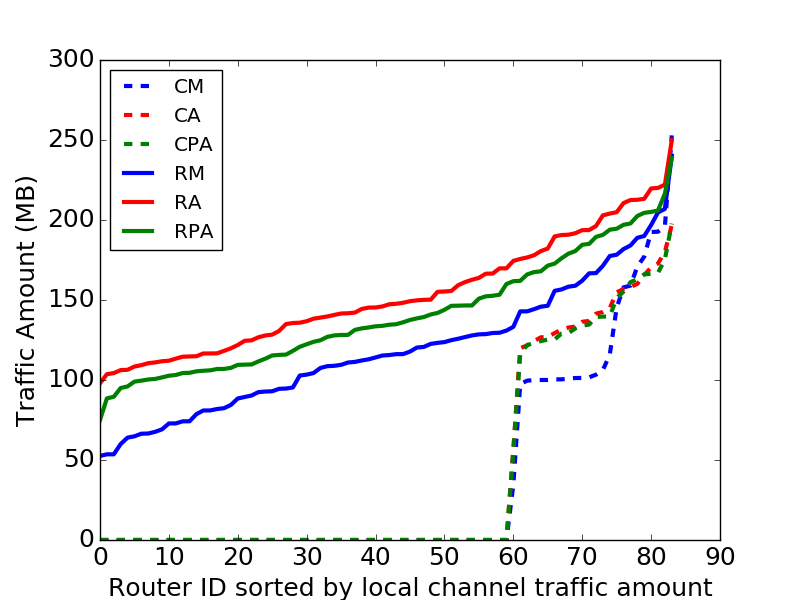
\includegraphics[height=1.5 in]{syn-wkld/cr/lc-traffic}
        \caption{CR Local Channel Traffic}
        \label{fig:syn-cr-lc-traffic}
    \end{subfigure}\\
    \centering
    \begin{subfigure}[t]{0.32\textwidth}
        \centering
        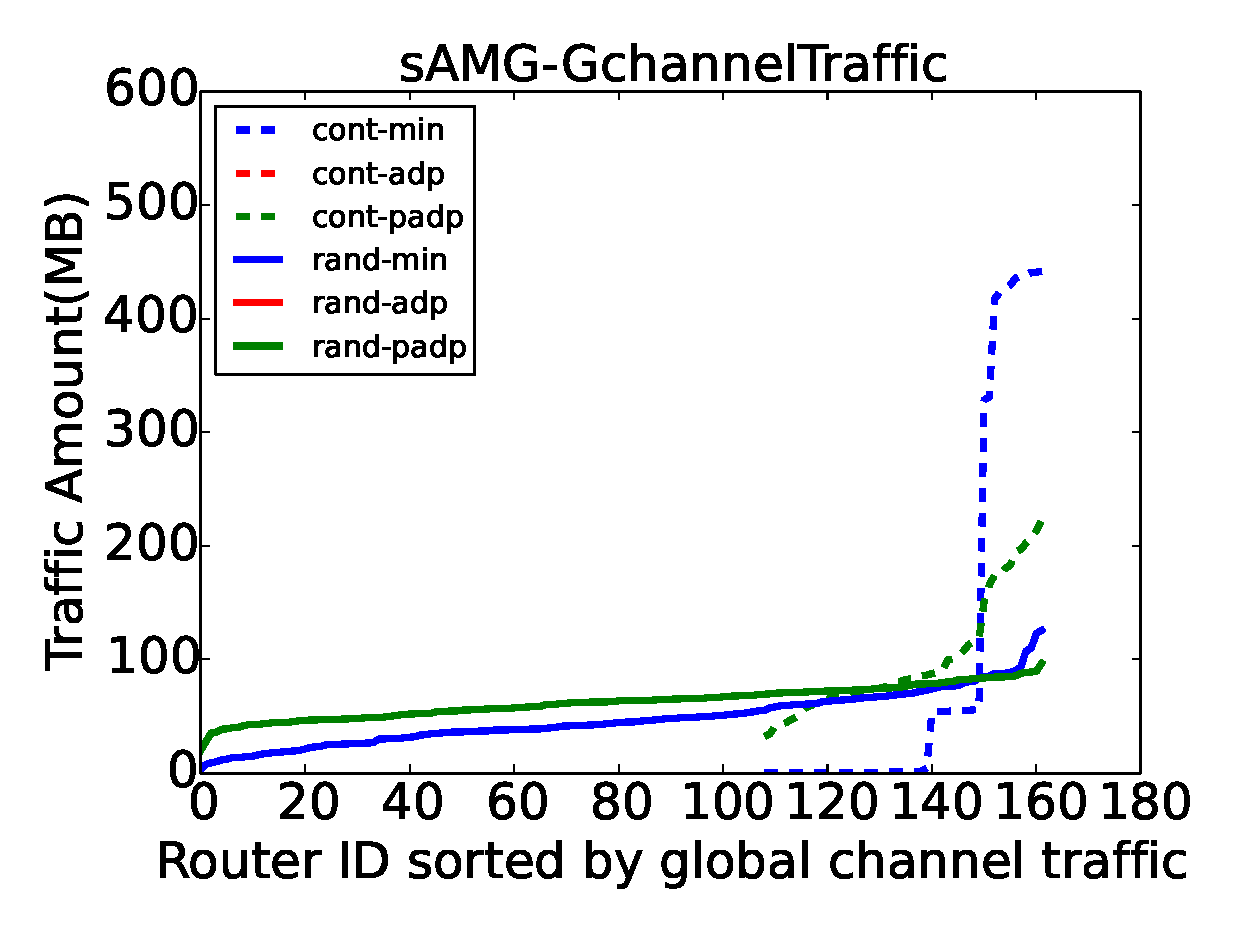
\includegraphics[height=1.5 in]{syn-wkld/amg10/gc-traffic}
        \caption{sAMG Global Channel Traffic}
        \label{fig:syn-samg-gc-traffic}
    \end{subfigure}\hfill
    \hspace{1em}%
    \begin{subfigure}[t]{0.32\textwidth}
        \centering
        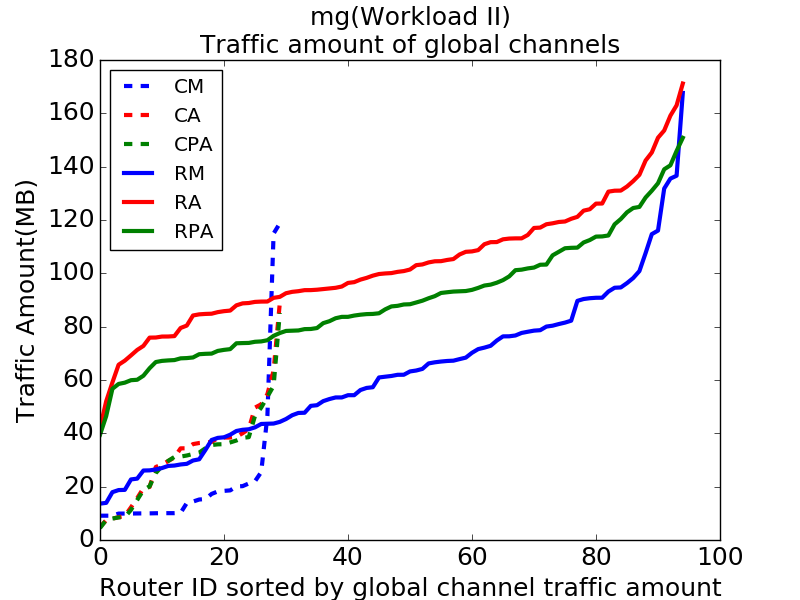
\includegraphics[height=1.5 in]{syn-wkld/mg/gc-traffic}
        \caption{MG Global Channel Traffic}
        \label{fig:syn-mg-gc-traffic}
    \end{subfigure}\hfill
    \begin{subfigure}[t]{0.32\textwidth}
        \centering
        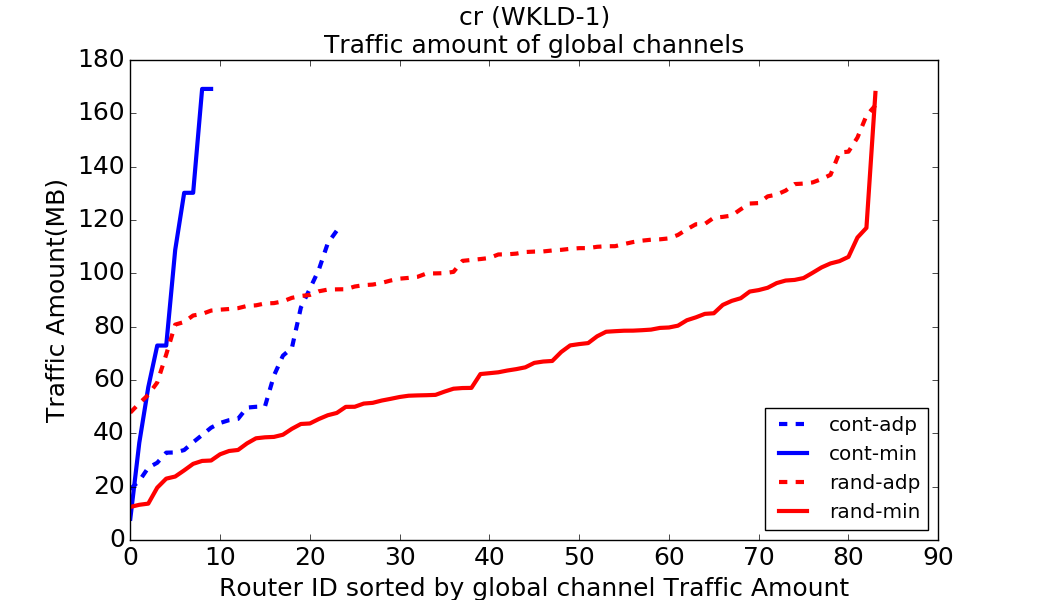
\includegraphics[height=1.5 in]{syn-wkld/cr/gc-traffic}
        \caption{CR Global Channel Traffic}
        \label{fig:syn-cr-gc-traffic}
    \end{subfigure}%
   \caption{Each Application Router Local and Global Channel Traffic.}
   \label{fig:syn-3app-gc-traffic}
\end{figure*}


\subsection{Key Finding}
Our study with synthetic workload confirms that the ``bully" behavior among concurrently running applications would happen when two conditions are satisfied.

\emph{First, the placement \& routing configuration allows network resource sharing between concurrently running applications. Random placement enables the router sharing and adaptive routing enables local and global channel sharing.}

\emph{Second, there are variance in terms of communication intensity between concurrently running applications. In workload \Rmnum{1}, AMG has the least amount of communication traffic compared with MultiGrid and CrystalRouter and it become the ``bullee". In workload \Rmnum{2}, sAMG has the most amount of communication traffic, which makes it the ``bully". }

We can stop this ``bully" by making either one of these conditions invalid. 


%\section{Summary}
%Based on the results we got from both real application traces and synthetic workload, we can make the following observations:
%
%\begin{itemize}
%    \item Random placement and adaptive routing can uniformly distribute workload traffic over the network, make the whole network load-balanced and hot-spots free. 
%    \item Random placement and adaptive routing can not guarantee QoS for each application in the workload. In order to reach load-balanced and hot-spots free, the traffic from congested routers will be redirected to other less busy routers. This will indulge the ``bully" that communication-intensive applications impose to their less intensive peers. 
%    \item Contiguous placement and minimal routing guarantee a consistent performance of each application. Although, contiguous placement and minimal routing usually results in local congestion and unbalanced network utilization, it can reduce the interference between concurrently running applications, thus prevent less communication-intensive application from being ``bullied" by its communication-intensive peers.
%\end{itemize}


%We believe choosing the ideal placement and routing strategies for workload running on dragonfly network should be based on application's communication intensity. The less intensive applications should avoid sharing network resource with other applications, reduce the possible interference. Contiguous placement and adaptive routing can guarantee the QoS for the less intensive applications, thus prevent the ``bully" from happening. 

%The communication-intensive applications tend to cause local congestion. It is preferable to enable communication-intensive applications to have extra network resource by sharing with other applications.  Random placement and adaptive routing can alleviate the local congestion by redirecting traffic to other less busy routers in the network. 

%So the ideal placement and routing strategies for workload running on dragonfly network should be like this. The communication-intensive applications should be randomly allocated over the system and adaptive routing should be used by these applications to alleviate the local congestion. On the other hand, less intensive application should get contiguous allocation, minimal routing should be used by these applications to avoid network sharing and reduce interference. 
 


\section{Related Work}
\label{sec:related work}

The impact of job placement to both system and application always catch researchers appetite \cite{dskinner} \cite{abhinav-sc13} \cite{jose-ipdps15}. Skinner et al. identified that network congestion could cause significant performance variability \cite{dskinner}. Bhatele et al. studied the performance variability of a specific application, p3FD, running on different production system \cite{abhinav-sc13}. They noticed that the application performance would keep consistent when it got compact allocation and exclusive network resource. Jokanovic et al. studied the impact of job placement to the workload and claimed that the key to reduce performance variability is to avoid network sharing \cite{jose-ipdps15}. 

Recently, several researchers have investigated the job placement and routing schemes on dragonfly network. Bogdan et al. proposed novel solution for mapping tasks of application that conforms to Nearest Neighbor communication pattern on dragonfly network \cite{hoefler-hpdc14}. Jain et al. conducted a comprehensive analysis of various job placement and routing scheme with regard to network link throughput on dragonfly network \cite{jain-sc14}. Their work is based on an analytical model and synthetic workload. Bhatele et al. used simulation to study the performance of synthetic workload under the different task mapping and routing schemes on two-level direct networks \cite{bhatele-sc11}.


Our work different from the previous works in the following ways. First, instead of using synthetic workload that generated based on predefined communication patterns, our simulation is driven by real application traces collected from production system. Second, not only we care about the workload performance, but also we pay attention to each individual application in the workload. We found that although random placement \& adaptive routing can improve the workload performance, some specific application in the workload may suffer performance degradation. Third, with the sophisticated simulation tool CODES, we can not only get applications communication information, but also the insight about the network status when application is running. The traffic and busy time of router's each link are valuable information for detailed analysis.

\section{Conclusion}
\label{sec:conclusion}

In this paper, we have conducted extensive study about application's behavior when running on dragonfly network with different job placement and routing configurations. We resorted to CODES, a high-fidelity HPC network simulation tool, and used three parallel scientific applications traces collected from production system to analysis the applications' behavior on network level. We found that when applications are running concurrently, although random placement can uniformly distribute the workload traffic over the network to reach load balance and hot-spots free for the network, the performance of certain application would be impaired. We identify this phenomenon as ``bully" between concurrently running applications, and the victim always being the less communication-intensive one. On the other hand, the contiguous placement tend to cause local congestion, however when coupled with adaptive routing, the configuration can guarantee the performance of ``bullee" application by limiting the network sharing between concurrently running peers. 

Due the presence of this ``bully", we suggest that when the batch scheduler make job placement for workload on dragonfly system, random placement shouldn't be the rule of thumb. Instead, the placement should made with consideration of jobs communication intensity. The less intensive application should get contiguous allocation coupled with adaptive routing, the intensive ones should get random allocation coupled with minimal routing. We believe the findings presented in this paper can illuminate a path to more efficient workload manager for future systems with dragonfly network.



% conference papers do not normally have an appendix



% use section* for acknowledgment
\ifCLASSOPTIONcompsoc
  % The Computer Society usually uses the plural form
  \section*{Acknowledgments}
\else
  % regular IEEE prefers the singular form
%   \section*{Acknowledgment}
\fi


The work at Illinois Institute of Technology is supported in part by U.S. National Science Foundation grants CNS-1320125 and CCF-1422009. This work is also supported by the U.S. Department of Energy, Office of Science, Advanced Scientific Computing Research, under Contract DE-AC02-06CH11357.


% trigger a \newpage just before the given reference
% number - used to balance the columns on the last page
% adjust value as needed - may need to be readjusted if
% the document is modified later
%\IEEEtriggeratref{4}


\bibliographystyle{IEEEtran}
\bibliography{./reference}  


 \vspace{5\baselineskip}
 
 \begin{framed}
 The submitted manuscript has been created by UChicago Argonne, LLC, Operator of Argonne National Laboratory ("Argonne").  Argonne, a U.S. Department of Energy Office of Science laboratory, is operated under Contract No. DE-AC02-06CH11357.  The U.S. Government retains for itself, and others acting on its behalf, a paid-up nonexclusive, irrevocable worldwide license in said article to reproduce, prepare derivative works, distribute copies to the public, and perform publicly and display publicly, by or on behalf of the Government.
 \end{framed}




% that's all folks
\end{document}


